\documentclass[12pt]{report}
\usepackage[utf8]{inputenc}
\usepackage[T1]{fontenc}
\usepackage{german}
\usepackage{geometry}                
\geometry{a4paper}                   
\usepackage{float}
\usepackage[parfill]{parskip}   
\usepackage{xifthen}
\usepackage{xstring}
\usepackage{graphicx}
\usepackage[usenames,dvipsnames,table]{xcolor}
\usepackage{amssymb}
\usepackage{epstopdf}
\usepackage{hyperref}
\usepackage{fancyhdr}
\usepackage{multirow}
\usepackage{listings}
\usepackage{tabularx} 
\usepackage{longtable}
\usepackage{booktabs} 	% Tabellenstyle

\renewcommand{\lstlistingname}{Code}
\renewcommand{\lstlistlistingname}{Codebeispiele}

\definecolor{javared}{rgb}{0.6,0,0}
\definecolor{javagreen}{rgb}{0.25,0.5,0.35}
\definecolor{javapurple}{rgb}{0.5,0,0.35}
\definecolor{javadocblue}{rgb}{0.25,0.35,0.75}
\definecolor{pblue}{rgb}{0.13,0.13,1}
\definecolor{pgreen}{rgb}{0,0.5,0}
\definecolor{pred}{rgb}{0.9,0,0}
\definecolor{pgrey}{rgb}{0.46,0.45,0.48}

\usepackage{listings}
\lstset{language=Java,
  showspaces=false,
  showtabs=false,
  breaklines=true,
  showstringspaces=false,
  breakatwhitespace=true,
  commentstyle=\color{pgreen},
  keywordstyle=\color{pblue},
  stringstyle=\color{pred},
  basicstyle=\ttfamily,
  moredelim=[il][\textcolor{pgrey}]{\$\$},
  moredelim=[is][\textcolor{pgrey}]{\%\%}{\%\%}
}

\lstdefinelanguage{JavaScript}{
  keywords={typeof, new, true, false, catch, function, return, null, catch, switch, var, if, in, while, do, else, case, break},
  keywordstyle=\color{blue}\bfseries,
  ndkeywords={class, export, boolean, throw, implements, import, this},
  ndkeywordstyle=\color{darkgray}\bfseries,
  identifierstyle=\color{black},
  sensitive=false,
  comment=[l]{//},
  morecomment=[s]{/*}{*/},
  commentstyle=\color{purple}\ttfamily,
  stringstyle=\color{red}\ttfamily,
  morestring=[b]',
  morestring=[b]"
}

\lstset{
   language=JavaScript,
   extendedchars=true,
   basicstyle=\footnotesize\ttfamily,
   showstringspaces=false,
   showspaces=false,
   numbers=left,
   numberstyle=\footnotesize,
   numbersep=9pt,
   tabsize=2,
   breaklines=true,
   showtabs=false,
   captionpos=b
}

\IfStrEq*{\languagename}{english}
	{
		\newcommand{\dalabel}{Diploma Thesis}
		\newcommand{\submittedlabel}{Submitted by}
		\newcommand{\datelabel}{Date}
		\newcommand{\supervisorlabel}{Supervisor}
		\newcommand{\projectpartnerlabel}{Project Partner}
	}
	{
		\newcommand{\dalabel}{Diplomarbeit}
		\newcommand{\submittedlabel}{Eingereicht von}
		\newcommand{\datelabel}{Datum}
		\newcommand{\supervisorlabel}{Betreuer}
		\newcommand{\projectpartnerlabel}{Projektpartner}
	}

\newcommand{\titleofthesis}{HomeDS}
\newcommand{\department}{Informatik} % Replace by your department

\newcommand{\firstauthor}{Andrej Sakal}
\newcommand{\firstauthorclass}{5CHIF}
\newcommand{\secondauthor}{Felix Hofmann}
\newcommand{\secondauthorclass}{5CHIF}

\newcommand{\duedateen}{April 4, 2018} % due date in english format
\newcommand{\duedatede}{4. April 2018} % due date in german format
\newcommand{\supervisor}{Thomas Stütz}


\begin{document}
\rhead{\includegraphics[scale=.9]{images/Logo.png}}
\cfoot{}
\begin{titlepage}
\thispagestyle{fancy}

\begin{center}

\vspace*{8em}

{\LARGE \dalabel}

\vspace{2em}

{\large Höhere Technische Bundeslehranstalt Leonding \\[.5em]
Abteilung für \department}

%\vspace{8em}
\vspace*{\fill}

{\Huge \titleofthesis}
\end{center}

%\vspace{8em}
\vspace*{\fill}

\begin{tabular}{ll}
\ifthenelse{\isundefined{\firstauthor}}{}{\submittedlabel: & {\bf \firstauthor, \firstauthorclass}}
\ifthenelse{\isundefined{\secondauthor}}{}{ \\[.5em] & {\bf \secondauthor, \secondauthorclass}}
\ifthenelse{\isundefined{\thirdauthor}}{}{ \\[.5em] & {\bf \thirdauthor, \thirdauthorclass}}
\ifthenelse{\isundefined{\fourthauthor}}{}{ \\[.5em] & {\bf \fourthauthor, \fourthauthorclass}}
 \\[.5em]
\datelabel: & {\bf \duedateen} \\[.5em]

\supervisorlabel: & {\bf \supervisor} \\[.5em]

\ifthenelse{\isundefined{\projectpartner}}{}{\projectpartnerlabel: & {\bf \projectpartner}}
\end{tabular}
\end{titlepage}

\section*{Declaration of Academic Honesty}
Hereby, I declare that I have composed the presented paper independently on my own and without any other resources than the ones indicated. All thoughts taken directly or indirectly from external sources are properly denoted as such.

This paper has neither been previously submitted to another authority nor has it been published yet. \\[1em]
Leonding, \duedateen \\[5em]
\ifthenelse{\isundefined{\firstauthor}}{}{\firstauthor}
\ifthenelse{\isundefined{\secondauthor}}{}{\kern-1ex, \secondauthor}
\ifthenelse{\isundefined{\thirdauthor}}{}{\kern-1ex, \thirdauthor}
\ifthenelse{\isundefined{\fourthauthor}}{}{\kern-1ex, \fourthauthor} \\[5em]

\begin{otherlanguage}{german}
\section*{Eidesstattliche Erkl�rung}
Hiermit erkl�re ich an Eides statt, dass ich die vorgelegte Diplomarbeit selbstst�ndig und ohne Benutzung anderer als der angegebenen Hilfsmittel angefertigt habe. Gedanken, die aus fremden Quellen direkt oder indirekt �bernommen wurden, sind als solche gekennzeichnet.

Die Arbeit wurde bisher in gleicher oder �hnlicher Weise keiner anderen Pr�fungsbeh�rde vorgelegt und auch noch nicht ver�ffentlicht. \\[1em]
Leonding, am \duedatede \\[5em]
\ifthenelse{\isundefined{\firstauthor}}{}{\firstauthor}
\ifthenelse{\isundefined{\secondauthor}}{}{\kern-1ex, \secondauthor}
\ifthenelse{\isundefined{\thirdauthor}}{}{\kern-1ex, \thirdauthor}
\ifthenelse{\isundefined{\fourthauthor}}{}{\kern-1ex, \fourthauthor} \\[5em]
\end{otherlanguage}

\begin{abstract}
Die HTL-Leonding besitzt schon einige Multimedia Systeme verstreut im ganzen Schulgeb�ude um Projekte, aktuelle News und �nderungen im Unterrichtsablauf anzuzeigen. Doch ein gro�er Schwachpunkt dieser Multimedia Systeme ist, dass der Prozess vom erstellen der Anzeige bis zum zuordnen welcher Bildschirm, welche Information anzeigen soll sehr kompliziert, und m�hselig ist. Sodass oftmals neue Informationen erst Versp�tet oder gar nicht angezeigt wird.

Unsere Diplomarbeit besch�ftigt sich mit dem erschaffen eines gemeinsames System zu entwickeln um einfach neue Supplierungen, Nachrichten oder Eilmeldungen auf allen Bildschirmen der HTL-Leonding anzuzeigen. Diese Systeme werden unter dem Begriff "Digital Signage System" zusammengefasst.




\tableofcontents

\chapter{Einleitung}
\section{Ausgangssituation}
Die HTL-Leonding besitzt schon einige Multimedia Systeme verstreut im ganzen Schulgeb�ude um Projekte, aktuelle News und �nderungen im Unterrichtsablauf anzuzeigen. Doch ein gro�er Schwachpunkt dieser Multimedia Systeme ist, dass der Prozess vom erstellen der Anzeige bis zum zuordnen welcher Bildschirm, welche Information anzeigen soll sehr kompliziert, und m�hselig ist. Sodass oftmals neue Informationen erst Versp�tet oder gar nicht angezeigt wird. 

\section{Ziele}
Die Ziele sind das die HTL Leonding den Sch�lern schneller Information oder Eilmeldungen auf den Multimedia System anzuzeigen.

\section{Overview}
Details of the diploma thesis have to be aligned between student and supervisor. This should be a basic structure to facilitate the first steps when students start to write their theses.

Never forget to add some illustrative images. Images must not be messed up with your normal text. They are encapsulated in floating bodies and referenced in your text. An example can be seen in figure~\ref{fig:sample}. As you can see, figures are placed by default on top of the page nearby the place where they are referenced the first time. Furthermore you can see that a list of figures is maintained automatically which can be included easily by typing the command \verb1\listoffigures1 into your document.

\begin{figure}
\begin{center}
	\includegraphics[scale=.5]{images/don_knuth.jpg}
\end{center}
	\caption{Don Knuth, the inventor of \TeX}
	\label{fig:sample}
\end{figure}

\section{Basic Terminology}
As usual the very basic terminology is briefly explained here. Most probably the explanations here only scratch a surface level. More detailed explanations of terminology goes into chapter~\ref{cha:theoretical-background}.

\section{Related Work and Projects}
Here a survey of other work in and around the area of the thesis is given. The reader shall see that the authors of the thesis know their field well and understand the developments there. Furthermore here is a good place to show what relevance the thesis in its field has.

\section{Structure of the Thesis}
%dsflkjas flaksjfl asdfj as lfjldsajflaksdjf sa dfjlasdkfj sadlfjasdklf als dfj l dfsdfsdfn chapter~\ref{cha:used-technologies} (\nameref{cha:used-technologies}) on page~\pageref{cha:used-technologies} we describe the used technologies.
Finally the reader is given a brief description what (s)he can expect in the thesis. Each chapter is introduced with a paragraph roughly describing its content.
\chapter{Digital Signage \& XIBO}
\section{Was ist Digital Signage?}\label{sec:digitalsignage}
Digital Signage, in Deutsch Digitales Schild, hat grundsätzlich die Aufgabe Inhalte die meist auf Plakaten oder Schildern angezeigt werden auf Bildschirmen anzuzeigen. Mithilfe von Digital Signage Systemen, soll das zeit- oder interaktionsgesteuerte Ändern von Inhalten auf den Bildschirmen einfach und übersichtlich gehalten werden siehe Abbildung \ref{img:digitalsignagehtlleonding}. Weiteres bietet Digital Signage ein breites Spektrum an Anwendungsbereichen. Digital Signage ist vor allem im Marketing Bereich ein sehr beliebtes Mittel, um ein neues Produkt oder eine Neuheit zu präsentieren. 

https://de.wikipedia.org/wiki/Digital_Signage#Anwendungsbeispiele:_2017.


\begin{figure}[H]
\centering
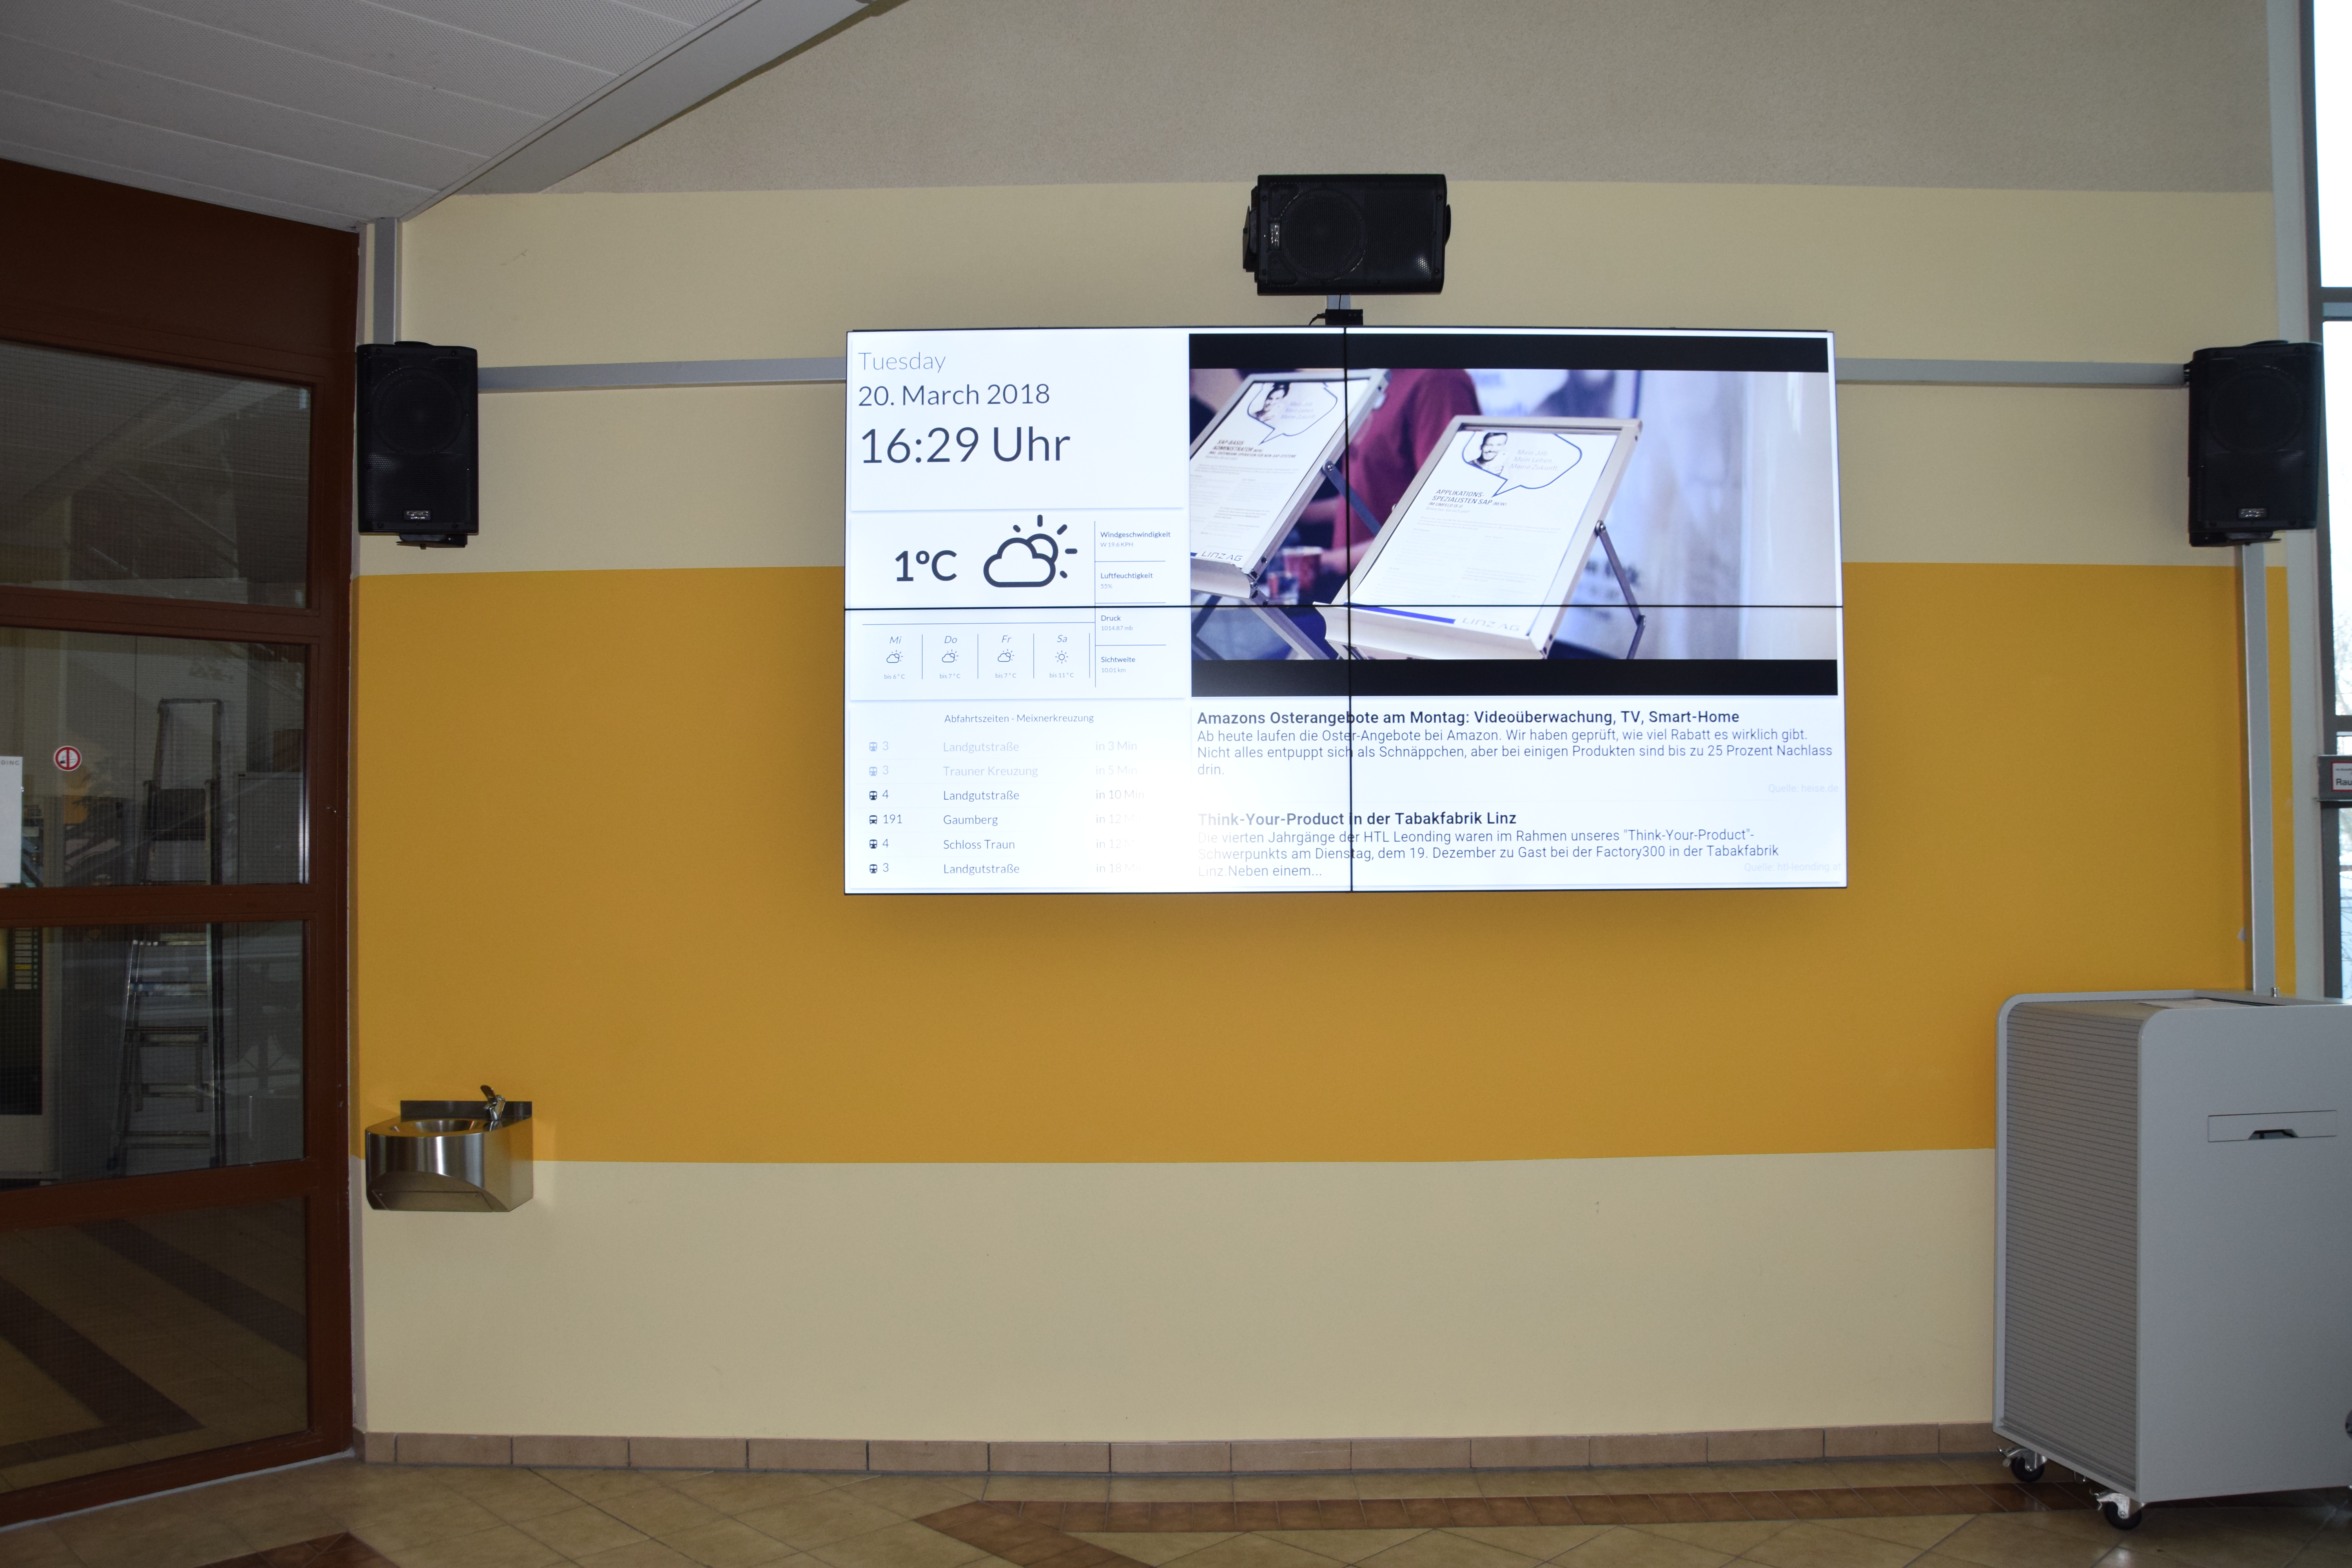
\includegraphics[width=1\textwidth]{images/02_XiboGrundlagen/Videowall.JPG}
\caption{Digital Signage in der HTL Leonding}
\label{img:digitalsignagehtlleonding}
\end{figure}

\section{Digital Signage Anwendungen}\label{sec:anwendungedigitalsignage}
Digital Signage hat keine Grenzen und kann vielfältig eingesetzt werden. Viele Konzerne nutzen Digital Signage für Marketing Zwecke, Produkte zu präsentieren oder oft auch nur als Lockmittel.

\section{Was ist XIBO?}\label{sec:xibo}
Das XIBO ist ein Open Source Digital Signage System entwickelt von der Spring Signage LTD. Das XIBO-System besteht aus vielen verschiedenen Komponenten. Das XIBO Paket besteht aus einem klassischen Server-Client Konstrukt. Der Server besteht aus drei Komponenten: das Content Managment System welches mithilfe von ZeroMq bei Änderung der Inhalte diese aktualisieren soll, einer Datenbank und einer Weboberfläche, die es dem Benutzer ermöglichen soll das System zu bedienen.

\section{Weboberfläche des XIBO}\label{sec:webpagexibo}
Das Steuerungszentrum des ganzen Signage System ist die Weboberfläche, die ganz einfach über einen Browser unter der Serveraddresse aufgerufen werden kann. Auf der Willkommensseite sind die wichtigsten Funktionen des Signage Servers dargestellt:

\begin{enumerate}
	\item {\em Kalender:} Mit der Kalender Funktion kann eingetragen werden zu welchem Zeitpunkt, welcher Inhalt, auf welchem Bildschirm angezeigt werden soll. Diese Funktion ist einer der wichtigsten und meist verwendeten. In dem Xibo-Kalender werden auch bereits eingetragene Aktivitäten angezeigt.

\begin{figur}
	\centering
\includegraphics[width=1\textwidth]{images/xibo-basics-calendar}
	\label{img:calendar}
	\caption{XBIO - Kalender}
\end{calendar}	
	
	\item {\em Layouts:} 
	Die Layout-Funktion ist einer der wichtigsten Komponenten des Signage Systems. Es beschäftigt sich mit dem Designen der Inhalte. Auf diese Funktion kommen wir noch einmal zurück.
	
	\item {\em Bibliothek:} 
	Die Bibliothek-Funktion ist zuständig für das Verwalten der Medien. Hier können Sie verschiedene Dateien hochladen.  Diese Medien können dann in Layouts eingebunden und angezeigt werden.
	
	\item {\em Benutzer:} 
	Im Menüpunkt Benutzer können neue Benutzer angelegt und bereits bestehende bearbeitet oder gelöscht werden. Dabei gibt es auch ein Rechte-System. Es können auch Datenmengenbegrenzungen pro Benutzer eingestellt werden.
	
	\item {\em Einstellungen:} 
	Der Menüpunkt Einstellungen gibt dem Nutzer die Möglichkeit, verschiedene Optionen zu wählen. So sind zum Beispiel die richtige Zeitzone, E-Mail Benachrichtigungen, wichtige Einstellungen, die für ein einwandfreies Funktionieren des Xibo-Servers zuständig sind. Aus den Einstellungen ist auch der CMS geheimer Schlüssel zu finden, der für die Authentifizierung der API Zugriffe zuständig ist herauszulesen.
\end{enumerate}

\section{Designen mit XIBO}\label{sec:designexibo}
Beim Designen von einem neuen Layout im XIBO, muss zuerst die Bildschirmauflösung ausgewählt und dem Layout ein passender Name zugewiesen werden, sowie optional auch eine Beschreibung. 

\textbf{Layout Maske}

\begin{calendar}
	\centering
\includegraphics[width=1\textwidth]{images/xibo-basics-designer}
	\label{img:designeLayout}
	\caption{XIBO-Layout designen}
\end{calendar}	

Dem Layout kann nun eine Region oder auch mehrere  hinzugefügt werden. Eine Region kann mehrere Widgets enthalten. Mit einem Doppelklick auf die Region kann ein Widget hinzugefügt werden. Es gibt viele verschiedene Arten von Widgets:

\begin{widgettypes}
	\item {\em Bibliothek:} Mit diesem Widget können Elemente aus der Medienbibliothek in der Region angezeigt werden. Dabei werden PowerPoint Formate, Video, Bilder und andere Medien Datentypen unterstützt.
	
	\item {\em Uhr:} 
	Dieser Widgettyp bindet eine Uhr in die Region ein. Es kann entweder eine Uhr im Analogen Stil oder Digitalen Stil ausgewählt werden.
	
	\item {\em DataSet:} 
	Das DataSet Widget ist sehr wichtig und zeigt grob gesagt nacheinander Daten aus einem Array mit Key, Value Paaren an.
	
	\item {\em Wheather:} 
	Das Wheather Widget, in Deutsch Wetter, zeigt das aktuelle Wetter an. Es kann eingestellt werden ob es anhand von den GPS-Daten des Bildschirmes die Wetterdaten anzeigen soll oder ein vorher definierter Ort für die Daten verwendet werden soll.
	
	\item {\em Flash:} 
	Mit dem Flash Widget können Flash Inhalte abgespielt werden.
	
	\item {\em HLS:} 
	Mit dem HLS Widget können HLS Video Streams angezeigt werden.
	
	\item {\em Image:} 
	Mit dem Image Widget können Bilder entweder aus der XIBO Bibliothek angezeigt oder neue hochgeladen werden.
	
	\item {\em Local Video:} 
	Mit dem Local Video Widget können Videos oder Streams angezeigt werden.
	
	\item {\em PDF:} 
	Mit dem PDF Widget können PDFs entweder aus der XIBO Bibliothek angezeigt oder neue hochgeladen werden.
	
	\item {\em PowerPoint:} 
	Mit dem PowerPoint Widget können PowerPoint Präsentationen entweder aus der XIBO Bibliothek angezeigt oder neue hochgeladen werden.

	\item {\em Text:} 
	Mit dem Text Widget können Texte angezeigt werden.
	
	\item {\em Ticker:} 
	Mit dem Ticker Widget können Texte animiert angezeigt werden. Dabei können diese Texte aus einem DataSet oder einem RSS Feed stammen.
	
	\item {\em Webpage:} 
	Mit dem Webpage Widget können Webseiten angezeigt werden.
\end{widgettypes}

Nachdem eines der Widgets erstellt wurde kann das Ergebnis des Layouts mit einer Layout Vorschau kurz überprüft werden.

\chapter{XIBO-Server}
\section{Beschreibung}
Als zentrale Steuereinheit wird ein XIBO-Server verwendet. Um diesen verwenden zu können, war es notwendig sich in die Dokumentation einzulesen und die API-Schnittstelle auszuprobieren. Die Website des Servers diente vorerst als Übungsumgebung. Dadurch wurde es leicht auch die einzelnen Funktionen, inklusive der Vorgangsweise, des Servers zu verstehen.
\cite{xibo-server}
\section{API-Schnittstelle}
Die API-Schnittstelle des XIBO-Servers ist mittels Swagger dokumentiert. Diese Dokumentation deckt die Grundfunktionalitäten und die Form der Anfragen ab. Da die Schnittstelle des Servers später als wesentliches Verbindungsstück zwischen der eigens entwickelten Steuerungssoftware und dem Server dient, war es nötig, diese gründlich zu testen und auch zu verstehen. Anfangs wurde dafür mit Postman gearbeitet. Um mit Postman die Requests testen zu können musste festgestellt werden, welche Codierung für den Request verwendet wird. Im Falle des XIBO-Servers wird ''application/x-www-form-urlencoded'' als Codierung verwendet. Die Anfragen an den Server wurden im Java Code durch die ''libary'' OkHttp3 übernommen.
\cite{swagger}
\cite{postman}
\cite{Okhttp3}
\section{Authentifizierung}
Bevor ein Client(im Zuge der Diplomarbeit handelt es sich um den Java-EE-Server) Anweisungen an den XIBO-Server in Form von Rest-Reqests übermitteln kann muss sich dieser mittels OAuth2 authentifizieren. Dazu benötigt der eine vom Server generierte Client\_ID.
\cite{oAuth2}

Die Parameter: 
\begin{itemize}
	\item {\em Client\_ID:} XIBO-Server Anwendungen neue Anwendung
	\item {\em Client\_Secret:}  XIBO-Server Anwendungen neue Anwendung
	\item{\em grant\_type:} Muss in der Form ''&grant\_type=client\_credentials''
\end{itemize}
müssen dem Server übermittelt werden um die Authentifizierung mit dem XIBO-Server durchzuführen. Dies geschieht unter der URL ''api\/authorize\/access\_token''.






HomeDS\HomeDsBackend\src\main\java\at\htl\utils\AuthentificationHandler.java

Zuerst wird ein Request-Body erstellt. Dieser hat folgende Parameter in der Form: 
 ''client\_id=<CLIENT\_ID>\&client\_secret=<CLIENT\_SECRET>\&grant\_type=
 client\_credentials''
, die im Body mitgegeben werden und als Format 'application/x-www-form-urlencoded'  haben. Anschließend werden dem Header noch der "content-type'' mit dem Wert ''application/x-www-form-urlencoded'' und der Parameter ''cache-control'' mit dem Wert ''no-cache'' hinzugefügt. Als Ergebniss der Anfrage bekommt der Client einen '' access\_token '', dieser ist nun bei jeder Anfrage notwendig um sich beim Server zu authentifizieren und es dem Client zu ermöglichen Daten abzurufen beziehungsweise weiterzugeben.





\chapter{Verwendete Technologien}
\section{Git und GitHub}
Um als Team dynamisch arbeiten zu können, verwenden wir Software zur Versionsverwaltung. Hierbei handelt es sich um Git. 
Github ist die verwendete Online-Plattform, auf der Benutzer ihre Projekte gratis als Repository speichern. Dies ermöglicht einfaches arbeiten im Team und verhindert in den meisten Fällen Zusammenführungskonflikte. Mittels Git lässt sich auch einfach zurückverfolgen welches Teammitglied welche Änderungen gemacht hat. Bei Bedarf ist es möglich diese Änderungen zurückzusetzen.

Verwendet wird GitHub für die gesamte Diplomarbeit, sowohl für die Versionsverwaltung der Dokumente, als auch die einzelnen Applicationen. Um sicherzustellen, dass keine Konflikte durch paralleles Arbeiten entstehen, wird in Branches gearbeitet. Diese Branches wurden erstellt, wenn ein neues Arbeitspaket begonnen wurde, zum Beispiel die Android-App.

Bild Github und verweis Git/GitHub

\section{Android}

Android ist ein Betriebssystem für mobile Endgeräte, spezialisiert auf Touch-Anwendungen. Ziel ist es das Endgerät möglichst intuitiv und flexibel bedienen zu können. Mit Android ist es möglich open-source Applicationen zu erstellen, welche ein großes Publikum erreichen. Google stellt hier seinen eigenen ''PlayStore'' zur Verfügung, in dem die Applikationen gratis oder auch gegen Entgelt erworben werden können.
Diese Aspekte open-source, frei erhältlich und das Erreichen großes Publikum, sind ausschlaggebend dafür, dass die Applicationen in Android implementiert wird. Als Programmiersprache wird Java verwendet.
\\
\section{Java Enterprise Edition}\label{sec:javaee}
Die Java Platform, Enterprise Edition oder abgekürzt auch Java EE ist die technische nähere Beschreibung einer Softwarearchitektur, die programmierte Java Anwendungen ausführt.
(weiter ausführen)

QUELLE: https://de.Wikipedia.org/wiki/Java_Platform,_Enterprise_Edition

\section{JSF - Java Server Faces}\label{sec:javaee}
JSF ist ein Java Enterprise Edition Framework, welches zur Entwicklung von Webanwendungen verwendet wird. JSF wurde als Nachfolger von JSP eingeführt um die Mischung von HTML Code und Java Code übersichtlicher zu gestalten. Ziel der JSF Vorgehensweise ist es Anwendungen in Komponenten zu teilen, welche im besten Fall wiederverwendbar sind.

\section{IntelliJ IDEA}
Herausgeber dieser Entwicklungsumgebung ist JetBrains. Durch diese IDE wird die Entwicklung des Java-EE-Backends unterstützt, wobei Java nicht die einzige Programmiersprache ist, die in IntelliJ verwendet werden kann. Andere Programmiersprachen, wie zum Beispiel Groovy und Kotlin, können in der IDE ebenfalls programmiert werden. Des weiteren gibt es eine Vielzahl an Tools wie zum Beispiel der direkte Zugang zu diversen Datenbanken, beispielsweise wie MySQL Datenbanken, oder die Integration von ''build automation tools'' wie bower oder grunt. Zudem sind verschiedenste Versionsverwaltungssysteme wie GutHub mit IntelliJ kompatibel und ebenfalls direkt über die Benutzeroberfläche der IDE verwendbar.

\section{Android Studio}
Android Studio ist eine von Google und JetBrains bereitgestellte integrierte Entwicklungsumgebung um Android Applikationen zu entwickeln. Grundgerüst für die Entwicklungsumgebung, ist die ''IntelliJ IDEA''. Zu dem können über Android Studio Emulatoren verschiedenster Android Geräte heruntergeladen und gestartet werden, damit erstellte Applikationen leicht zu probieren sind. Zusätzlich bietet Android Studio GitHub Integration und einen großen Umfang an Werkzeugen und Testmöglichkeiten.
  
\chapter{HomeDS - Server}
\section{Einleitung}\label{sec:einleitung}
Im Rahmen der Diplomarbeit wird neben dem XIBO-Server ein eigen Programmierter Java Enterprise Edition Server eingesetzt. Aufgrund der hohen Komplexität des Signage-Servers aber relativ dünn dokumentierten API-Schnittstellen und begrenzten technischen Möglichkeiten muss ein eigen programmierter Server eingesetzt werden. Dieser wird die Kommunikation vom Signage Server zur Android App erleichtern.  
 
\section{Java Enterprise Edition}\label{sec:javaee}
Java Platform, Enterprise Edition, oder abgekürzt auch Java EE ist die technische nähere Beschreibung einer Softwarearchitektur die Java Programmierte Anwendungen ausführt.
(weiter ausführen)

QUELLE: https://de.Wikipedia.org/wiki/Java_Platform,_Enterprise_Edition
 
\section{Anforderungen an den HomeDS Server}\label{sec:homeds}
Der JavaEE Server soll die verschiedenen komplizierten Abläufe des XIBO-Servers vereinfachen. Die verschiedenen Zugriffe mittels REST die eigentlich direkt auf den XIBO laufen sollen werden über den JavaEE Server verwaltet. Dies hat insofern Vorteile da die komplizierten und meist mit viel Aufwand verknüpften Authentifizierungen wegfallen. Somit können ohne Probleme neue Funktionen hinzugefügt werden und ohne Probleme an neue Anforderungen angepasst werden.
 
\section{Funktionen des HomeDS Server}\label{sec:homedsfunction}
Der JavaEE Server verfügt über eine eigene MySQL Datenbank. Diese wird gebraucht um die "DataSets" aus dem Signage-Server zwischen zu speichern. Dies ist insofern erforderlich da die Aufgabenstellung erfordert die Datensätze entweder nur ab einem bestimmten Datum im Layout anzuzeigen oder bis zu einem bestimmten Datum diese angezeigt werden dürfen. 
 
\section{DataSet mit Ablaufdatum}\label{sec:datasetexpiredate}
Einer der wichtigsten Funktionen des Servers ist das hinzufügen, ändern und löschen vom DataSet. Da der Digital Signage Server über keine Felder wie Start- und Enddatum verfügen.

Die Logik ist simple der Benutzer kann Start- und Enddatum eingeben für jeden einzelnen DataSet eingeben. Und erst wenn das Datum genau in diesem Zeitintervall inklusive den Grenzen liegt wird das DataSet an den Xibo mittels API-Schnittstelle weitergegeben. 

\begin{lstlisting}
if (dataset.isActive() == false && (dataset.getFromDate().minusDays(1)
        .isBefore(LocalDate.now()))) {
    try {
        //if succesfull added then set active true and add id
        if ((id=dataSetApi.addDataSetField(dataset)) > 0) {
            dataset.setDataRowId(id);
            dataset.setActive(true);
            dataSetFieldFacade.save(dataset);
        }
    } catch (NoConnectionException e) {
        // Catch Exception
    }
}
\end{lstlisting}

Die Überprüfung ob die DataSets aus der Server-Datenbank im Zeitintervall liegen wird mittels eines "TimeSchedule" jeden Tag um 01:00 Uhr durchgeführt. Falls dieser dann im Intervall liegt wird der DataSet an den XIBO Signage Server gesendet. Diese Überprüfung beinhaltet auch das FromDate dies löscht bei überschreiten des Bis-Datums das DataSet aus dem Digital Signage heraus. 

Die Überprüfung ob das Startdatum heute oder vor dem heutigem Datum wird mithilfe der Java Annotation @Schedule realisiert. (siehe Codeausschnitt) 


 
\begin{enumerate}
  \item {\em :} Mit der Kalender Funktion kann eingetragen werden zu welchen Zeitpunkt welcher Inhalt auf welchem Bildschirm angezeigt werden soll. In dem Xibo-Kalender werden auch bereits eingetragene Aktivitäten angezeigt.
 
\begin{calendar}
  \centering
\includegraphics[width=1\textwidth]{images/xibo-basics-calendar}
  \label{Calendar}
\end{calendar}  
  
  \item {\em Layouts:} 
  Die Layout Funktion ist einer der wichtigsten Komponenten des Signage Systems es beschäftigt sich mit dem designen der Inhalte. Auf diese Funktion kommen wir noch einmal zurück
  
  \item {\em Bibliothek:} 
  Die Bibliothek Funktion ist zuständig für das Verwalten der Medien. Hier können Sie verschiedene Dateien hochladen.  Diese Medien können dann in Layouts eingebunden und angezeigt werden.
  
  \item {\em Benutzer:} 
  Im Menüpunkt Benutzer können neue Benutzer angelegt werden und bereits bestehende bearbeitet oder gelöscht werden. Dabei gibt es auch ein Rechte-System. Es könne auch Datenmengen Begrenzungen pro Benutzer eingestellt werden.
  
  \item {\em Einstellungen:} 
  Der Menöpunkt Einstellung gibt dem Nutzer die Möglichkeit verschiedene Optionen einzustellen. So sind zum Beispiel die richtige Zeitzone, E-Mail Benachrichtigungen wichtige Einstellungen die für ein Einwandfreies funktionieren des Xibo-Servers zuständig wichtig sind.
\end{enumerate}
 
\section{Designen mit XIBO}\label{sec:designexibo}
Beim Designen von einem neuen Layout im XIBO muss zuerst die Bildschirm auflösung ausgewählt werden. Und dem Layout ein passender Name zugewiesen werden sowie optional auch eine Beschreibung. 
 
\textbf{Layout Maske}
 
\begin{calendar}
  \centering
1 file change in working directory
View change
commit:c95ae5
WIP on master: Auto stash before merge of "master" and "origin/master"

\chapter{Android Application}
\section{Einleitung}

\begin{figure}[H]
\centering
\includegraphics[width=1.0\textwidth]{images/06_AndroidApp/06_SystemArch}
\caption{Die Android Applikation dient zur mobilen Benutzung}
\end{figure}
\\
Um eine höchst mögliche Reichweite an Endgeräten zu erzielen, wurde eine Android Applikation entwickelt, mit der die wichtigsten Funktionen abgedeckt werden. Zum Beispiel das Wechseln der DataSets des XIBO-Servers. Wichtig war es die Applikation möglichst einfach und leicht bedienbar zu gestalten, um auch Erstbenutzern die Bedienung zu erleichtern. 
Prototyp für die aktuelle Applikation war eine Anwendung für Android, die direkt mit dem Digital Signage Server kommuniziert. Es stellte sich heraus, dass das Steuern des Servers direkt über eine Applikation auf Android Basis viel zu umständlich ist, wurde eine Browser Applikation entwickelt, welche über das ''HomeDsBackend''(Java-EE-Server) kommuniziert, um das Funktionsspektrum zu erweitern und die Applikation möglichst kompakt zu gestalten. Beispielsweise ist es durch diese Aufteilung nicht mehr nötig eine Datenbank in der Applikation zu haben. Somit erleichtert es auch Applikationen für andere Betriebssysteme zu implementieren. 
\section{Anforderungen}
\\
\begin{figure}[H]
\centering
\includegraphics[width=1.0\textwidth]{images/06_AndroidApp/06_AndroidArch}
\caption{Fluss Diagramm der Android Anwendung}
\label{fig:mediaNav}
\end{figure}
\\
Die Anforderungen an die Android Applikation weichen von den Anforderungen an das ''Backend'' leicht ab, da das ''Backend'' die gesamte Zeitsteuerung- und Datenbankfunktionalität übernimmt. Es besteht die Möglichkeit, den Server über die Website des ''Backend'' zu steuern, beziehungsweise über die Applikation auf Android Basis. 
\begin{itemize}
	\item {\em Eilmeldungen:} Dem Benutzer soll es möglich sein Nachrichten in einem Ticker auf den Bildschirmen anzuzeigen.
	
	\item {\em Medien Wiedergabe:} Medien die Lokal am Digital Signage Server liegen sollen abgespielt werden können.
		
	\item {\em Authentifizierung automatisieren (Prototyp Applikation):} Die Authentifizierung am Digital Signage Server soll automatisiert werden, um nicht vom Benutzer durchgeführt werden zu müssen.  		
\end{itemize}
\section{Struktur}
\begin{itemize}
	\item {\em activity:} Alle Activities die für die Anwendung benötigt werden. Als Beispiel die MainActivity
	
	\item {\em adapter:} Hier befinden sich alle Adapter für die RecyclerViews.
	
	\item {\em apiClient:} Beinhaltet die Klasse ''RequestHelper'' mit der die Anfragen an den Digital Signage Server beziehungsweise an das HomeDsBackend vereinfacht werden.
	
	\item {\em entity:} Jene Klassen die als Models für die Anwendung benötigt werden. 
		
	\item {\em enumeration:} Enumerationen welche die Android Basierte Applikation verwendet. Zum Beispiel das ''RequestTypeEnum''.
	
	\item {\em fragment:} Alle Fragments die für das User Interface benötigt werden. Beispiel hierfür ist das Fragment ''NewsOverviewFragment'', welches alle DataSets die am Server sind anzeigt.
	
	\item {\em viewholder:} Beinhaltet alle ''ViewHolder'' die für die Verschiedenen ''RecyclerViews'' benötigt werden. 		
\end{itemize}
\section{Benutzerhandbuch}
\subsection{Startseite}
Auf der Einstiegsseite der Applikation ist ein Feld mit dem Serverstatus zu sehen sollte dieses Rot eingefärbt sein gibt es Verbindungsprobleme zum Server(die Applikation kann keine Daten vom Server erhalten oder Daten an den Server senden) andernfalls kann mit der Benutzung fortgefahren werden, des Status wird grün Angezeigt. Die Funktion der Beiden Buttons wird im weiteren velauf des Benutzerhandbuchs erklärt.(Siehe Abbildung \ref{img:onlineOffline})
\\
\begin{figure}[H]
    \centering
    \subfloat{{\includegraphics[width=6cm]{images/06_AndroidApp/06_StatusOnline}}}%
    \qquad
    \subfloat{{\includegraphics[width=6cm]{images/06_AndroidApp/06_StatusOffline}}}%
    \caption{Startseite mit Status Element Online/Offline}
    \label{img:onlineOffline}
\end{figure}
\\
\subsection{Abspielen von Medien auf gewünschten Bildschirmen}
Das Abspielen von Medien wird im Navigationstab ''Play Media'' abgewickelt, des weiteren befindet sich auf der Startseite ein Button über den direkt zu dieser Sektion navigiert werden kann.(Siehe Abbildung \ref{fig:mediaNav})
\\
\begin{figure}[H]
\centering
\includegraphics[scale=0.35]{images/06_AndroidApp/06_mediaNavigation}
\caption{Startseite mit markierten Navigationselementen}
\label{fig:mediaNav}
\end{figure}
\\
Wurde noch kein Display gewählt, auf dem das Medium abgespielt werden soll, erscheint zu beginn eine Auswahlmaske für die Bildschirme die verfügbar sind. Nach Auswahl einer Anzeige navigiert die Applikation automatisch zur Medienübersicht. (Siehe Abbildung \ref{fig:dispNav})
\\
\begin{figure}[H]
\centering
\includegraphics[scale=0.35]{images/06_AndroidApp/06_displayChoice}
\caption{Liste mit verfügbaren Displays}
\label{fig:dispNav}
\end{figure}

Ist bereits ein Bildschirm ausgewählt wird direkt eine Übersicht der abspielbaren Medien angezeigt. Im rechten oberen Teil der Ansicht ist der Gewählte Bildschirm zu sehen und über einen Button wird die Bildschirmauswahl angezeigt.(Siehe Abbildung \ref{fig:mediaOv})
\begin{figure}[H]
\centering
\includegraphics[scale=0.35]{images/06_AndroidApp/06_displayTextAndButton}
\caption{Ausgewählter Bildschirm und Button für die Auswahl}
\label{fig:mediaOv}
\end{figure}
\\
Sortieren der angezeigten Medien ist über einen Spinner im linken oberen Teil der Medien Übersicht möglich durch Berührung der Anzeigefläche erscheint die Auswahl der Sortiervorschläge.(Siehe Abbildung \ref{fig:spinner})
\begin{figure}[H]
\centering
\includegraphics[scale=0.35]{images/06_AndroidApp/06_TagChoice}
\caption{Spinner mit Tags zur Sortierung}
\label{fig:spinner}
\end{figure}
\\
Um ein in der Liste angezeigtes Medium abzuspielen muss der Play-Button im rechten teil des Listenelements gedrückt werden. Wurde der Button betätigt wird das Medium auf der gewählten Anzeige abgespielt.(Siehe Abbildung \ref{fig:playBut})
\begin{figure}[H]
\centering
\includegraphics[scale=0.35]{images/06_AndroidApp/06_playMedia}
\caption{Play Button um Medium abzuspielen}
\label{fig:playBut}
\end{figure}
\\
\subsection{Meldungen Anzeigen}
Um eine Meldung anzuzeigen muss zum ''DataSet'' Tab gewechselt werden dies ist auch über eine Schaltfläche auf der Startseite von statten gehen. (Siehe Abbildung \ref{fig:06_dataSetNavigation})
\begin{figure}[H]
\centering
\includegraphics[scale=0.35]{images/06_AndroidApp/06_dataSetNavigation}
\caption{Startseite mit Navigationselementen}
\label{fig:06_dataSetNavigation}
\end{figure}
\\
Die in der Ansicht zu sehende Liste enthält alle aktiven und  inaktiven Meldungen die auf den Anzeigen wiedergegeben werden beziehungsweise werden können.
(Siehe Abbildung \ref{fig:06_DataSetsToSHow}) 
\\
\begin{figure}[H]
\centering
\includegraphics[scale=0.1]{images/06_AndroidApp/06_DataSetsToSHow}
\caption{Am HomeDsBackend vorhandene DataSets}
\label{fig:06_DataSetsToSHow}
\end{figure}

\\
Durch auswählen eines der Listenelemente öffnet sich einer Detailansicht über die die Informationen der Meldung verändert werden können zum Beispiel der Titel oder der Anzeigezeitraum. Wird der FloatingActionButton im unteren rechten teil der Ansicht gedrückt so öffnet sich ein Detailfenster welches noch keine Daten eingetragen hat um eine neue Meldung zu erstellen. (Siehe Abbildung \ref{fig:06_NewNewsEdit})
\\
\begin{figure}[H]
    \centering
    \subfloat{{\includegraphics[width=6cm]{images/06_AndroidApp/06_NewNewsEdit}}}%
    \qquad
    \subfloat{{\includegraphics[width=6cm]{images/06_AndroidApp/06_EditNews}}}%
    \caption{Anzeige für ein neues/zu veränderndes DataSet}
    \label{fig:06_NewNewsEdit}
\end{figure}
\\
Vorgenommene Änderungen oder neu erstellte Meldungen können mittels Save Button übernommen werden. Dieser befindet sich im unteren teil der Detailansicht. Nach speichern einer Meldung navigiert die Applikation wieder auf die Übersicht der Meldungen.(Siehe Abbildung \ref{fig:06_EditNewsSaveButton})

\begin{figure}[H]
\centering
\includegraphics[scale=0.35]{images/06_AndroidApp/06_EditNewsSaveButton}
\caption{Markierter speichern Button}
\label{fig:06_EditNewsSaveButton}
\end{figure}

\subsection{Strukturübersich}
Ist es von Nöten eine detailierte Übersicht über die am Server liegenden Layouts zu bekommen kann dies über den Navigationstab ''Structure Plan'' getan werden.(Siehe Abbildung \ref{fig:06_EditNewsSaveButton}) 
\\
\begin{figure}[H]
\centering
\includegraphics[scale=0.35]{images/06_AndroidApp/06_EditNewsSaveButton}
\caption{Markierte Liste mit Layouts und Navigationstab}
\label{fig:06_EditNewsSaveButton}
\end{figure}
\\
Die Liste zeigt alle am Server befindlichen Layouts durch klicken einer der Listenelemente navigiert die Applikation zu einer Detailansicht des Layouts.(Siehe Abbildung \ref{fig:06_StructureNavigationToDetail})
\\
\begin{figure}[H]
\centering
\includegraphics[scale=0.35]{images/06_AndroidApp/06_StructureNavigationToDetail}
\caption{Markiertes Element um auf die Detailansicht zu gelangen}
\label{fig:06_StructureNavigationToDetail}
\end{figure}
\\
Die Detailansicht eines Layouts zeigt die Grunddaten eines Layouts wie zum Beispiel die ID oder die Besitzer ID. Des weiteren werden alle unterelemente beispielsweise Widget's angezeigt. Dargestellt wird der JSON-String des Layouts.
(Siehe Abbildung \ref{fig:06_StructureDetail})
\\
\begin{figure}[H]
\centering
\includegraphics[scale=0.35]{images/06_AndroidApp/06_StructureDetail}
\caption{Markierte Details des Layouts}
\label{fig:06_StructureDetail}
\end{figure}
\\
\section{MainBottomNavigationActivity und OverviewFragment}
\subsection{MainBottomNavigationActivity}
\\
\begin{figure}[H]
\centering
\includegraphics[width=1.0\textwidth]{images/06_AndroidApp/06_AndroidArchMainBottomNavigationActivity}
\caption{Stellung des MainBottomNavigationFragemt in der Android Applikation}
\label{fig:mediaNav}
\end{figure}
\\
Die ''MainBottomNavigationActivity'' ist die Einzige ''Activity'' die in der Android Applikation benötigt wird. Hauptaufgabe der ''MainBottomNavigationActivity'' ist es, zwischen den einzelnen ''Fragments'' zu navigieren. Enthalten sind dazu jene Methoden, welche mit dem ''SupportFragmentManager'' die einzelnen Fragments im ''container\_main'' austauschen. Der ''container\_main'' ist ein ''ConstraintLayout'' welches in der zur ''MainActivity'' gehörenden Layout Ressource ''activity\_main.xml'' mit der Identifikationsnummer ''container\_main'' und  belegt wurde. Zudem wird die Klasse durch das Interface ''AppCompatActivity'' erweitert und implementiert die ''OnFragmentInteractionListener'' der Fragmente die in der Applikation verwendet werden. 
\
Im unteren Teil der ''Activity'' befindet sich eine Navigationsleiste. Diese ist zuständig für das wechseln zwischen den einzelnen Fragmenten mit folgenden Navigationspunkten: 

\begin{itemize}
	\item {\em Home:} Jener Menüpunkt der die Startseite der Applikation beinhaltet.
	\item {\em DataSet:} Ist zuständig für die Verwaltung der ''DataSets''.
	\item{\em Medium abspielen:} Beinhaltet die Fragmente die benötigt werden um Medien auf der gewünschten anzeige abzuspielen.
	\item {\em Strukturplan:} Bietet eine Übersicht über die Struktur der am Server liegenden Layouts.
\end{itemize}
\subsubsection{onCreate}
Hier wird die ''MainBottomNavigationActivity'' als ''ContentView'' gesetzt, zudem wird mittels ''SupportFragmentManager'' das ''HomeScreenFragment'' dem ''container\_main'' zugewiesen und angezeigt. Das Feld Display wird neu instantiiert. Die statische Variable ''instance'', vom Datentyp ''MainBottomNavigationActivity'', wird auf die aktuelle Instanz der Klasse zugewiesen. Die ''BottomNavigationBar wird mit werten belegt und ein ''OnNavigationItemSelectedListener'' gesetzt um durch die Applikation navigieren zu können.
\begin{lstlisting}[language=Java,caption={Zuweisung von Variablen und Navigationbar}]
setContentView(R.layout.
	activity_main_bottom_navigation);
mainActivityBottomNavigation = this;
openHomeScreenFragment();
display = new Display();
 
navbar = findViewById(R.id.navigation_bar);
navbar.setOnNavigationItemSelectedListener(
	new BottomNavigationView.
   	OnNavigationItemSelectedListener() {
    	@Override
     	public boolean onNavigationItemSelected(
     				@NonNull MenuItem item) {
     		item.setChecked(true);
        	switch (item.getItemId()) {
        		case R.id.editDatasetNavBar:
            		openNewsOverview();
                	break;
            	case R.id.playMediaNavBar:
                	if (display.getDisplay() == null){
                	openChooseDisplayFragment();
                	}else {
                	openMediaOverviewFragment();
                	}
                	break;
            	case R.id.homeScreenNavBar:
                	openHomeScreenFragment();
                	break;
            	case R.id.structurePlanNavBar:
                	openStructurePlanFragment();
                	break;
                	}
          	return false;
        }
	});
\end{lstlisting}	
\subsubsection{getInstance}
 Ist der ''Getter'' für die statische Variable ''instance'' und übergibt die aktuelle Instanz der Klasse.
\begin{lstlisting}[language=Java,caption={Getter für aktuelle Instanz der Activity}]
public static MainActivityBottomNavigation
	 getInstance() {
     return mainActivityBottomNavigation;
}
\end{lstlisting}
\subsubsection{Fragment-Austausch-Methoden}
 Sind jene Methoden die für das Austauschen der einzelnen ''Fragments'' im ''container\_main'' zuständig sind. Dies geschieht mittels ''SupportFragmentManager'' welcher immer die ''Fragments'' im ''container\_main'' anzeigt und dem ''BackStack'', welcher für die Rückwerts Navigation (mittels retour Knopf des Mobilen Endgerätes) in der Applikation zuständig ist,  hinzufügt. Manche Methoden übergeben zudem noch ein ''Bundle'' an das erstellte ''Fragment'', welches Objekte enthält die in nächsten ''Fragment'' benötigt werden. Erkennungsmerkmal dieser Methoden ist das englische Verb ''open'' am beginn des Methodennamens. Als Namensbeispiel hierfür wird die Methode ''openNewsEditFragment'' herangezogen.
\begin{lstlisting}[language=Java,caption={Beispiel für Fragment-Austausch-Methode}]
public void openEditNewsFragment(DataSetDataField news) {
Bundle bundle = new Bundle();
bundle.putSerializable("data", news);
NewsEditFragment newsEditFragment =
    new NewsEditFragment();
newsEditFragment.setArguments(bundle);
FragmentManager fm = getSupportFragmentManager();
fm.beginTransaction().replace(
    R.id.container_display, 	
    newsEditFragment,"actEdit")
    .addToBackStack("actEdit").commit();
}
\end{lstlisting}
\subsection{HomeScreenFragment}
\\
\begin{figure}[H]
\centering
\includegraphics[width=1.0\textwidth]{images/06_AndroidApp/06_AndroidArchHomeScreen}
\caption{Stellung des HomeScreenFragmnet in der Android Applikation}
\label{fig:mediaNav}
\end{figure}
\\
Der Einstiegspunkt der Applikation ist das ''HomeScreenFragment''. Es zeigt den Serverstatus an, dieser wird über einen ''REST-Request'' vom Java-EE-Server abgefragt. Den Hauptanteil des Fragments bilden die beiden Navigations-Buttons ''Median abspielen'' und ''Eilmeldungen anzeigen''. Durch klicken dieser Buttons öffnen sich die dazugehörigen Fragmente ''NewsOverviewFragment'' und ''MediaOverviewFragment''.
\\
Die Layout Ressource des ''HomeScreenFragment'' enthält zwei Buttons und ein ''ConstaintLayout''. Dieses ''ConstraintLayout'' beinhaltet wiederum eine ''TextView'' und zwei ''ImageViews''. In der ''onCreate'' Methode des Fragments werden als erstes die Anzeigeelemente neu deklarierten Variablen zugewiesen und im ''ConstraintLayout'' wird der Serverstatus auf View standardmäßig als Offline angezeigt und die Buttons deaktiviert.
\begin{lstlisting}[language=Java,caption={Initialisieren der Variablen im HomeScreenFragment }]
Button btPlayMedia = v.findViewById(R.id.btPlayMedia);
Button btShowNews = v.findViewById(R.id.btShowNews);

btPlayMedia.setEnabled(false);
btShowNews.setEnabled(false);
    
ImageView ivUp = v.findViewById(R.id.ivServerUp);
ivUp.setVisibility(View.INVISIBLE);
    
ImageView ivDown = v.findViewById(R.id.ivServerDown);    
ivDown.setVisibility(View.VISIBLE);
    
ConstraintLayout clServerStatus = 
    v.findViewById(R.id.cl_serverStatus);
clServerStatus.setBackgroundColor(
    ContextCompat.getColor(
    this.getContext(), R.color.serverDown));
}
\end{lstlisting}
Im folgenden Schritt wird über einen ''GET-Request'' die Uhrzeit des XIBO-Servers über den Java-EE-Server abgefragt. Wird eine Uhrzeit vom erhalten, so wird im ''ConstraintLayout'' des Server Status auf online gesetzt und das dazugehörige Bild angezeigt und die Buttons werden freigegeben. Erhält man keine Antwort bleibt die Anzeige unverändert.

\begin{lstlisting}[language=Java,caption={Status Request im HomeScreenFragment}]
rh.executeRequest(RequestTypeEnum.GET, null,
	MainActivityBottomNavigation.getInstance()
	.url + "/status/", () -> {   
    MainActivityBottomNavigation.getInstance()
    .runOnUiThread(() -> {
      	if (rh.getResponseCode() == 200) {
        	
           	ivUp.setVisibility(View.VISIBLE);
            ivDown.setVisibility(View.INVISIBLE);
                
            clServerStatus.setBackgroundColor(
           	ContextCompat.getColor(this.getContext(),
           	R.color.serverUp));
                	
            btPlayMedia.setEnabled(true);
            btShowNews.setEnabled(true);
                    
         }else {
         	ivDown.setVisibility(View.VISIBLE);
                    
            clServerStatus.setBackgroundColor(
            	ContextCompat.getColor(this.getContext(),
                R.color.serverDown));
            }
    });
});
\end{lstlisting}
Um die Navigation über die erstellten Buttons zu ermöglichen wird ein ''OnClickListener'' Implementiert.
\begin{lstlisting}[language=Java,caption={OnClickListener für die direkte Navigation über Buttons im HomeScreenFragment}]
btPlayMedia.setOnClickListener(
	new View.OnClickListener() {
            
    	@Override
        public void onClick(View view) {
            MainActivityBottomNavigation.
            getInstance().navbar
            .setSelectedItemId(R.id.playMediaNavBar);
        }
     });
\end{lstlisting}
\section{DataSet Verwaltung}
\\
\begin{figure}[H]
\centering
\includegraphics[width=1.0\textwidth]{images/06_AndroidApp/06_AndroidArchShowNews}
\caption{Stellung der DataSet Verwaltung in der Android Applikation}
\label{fig:mediaNav}
\end{figure}
\\
Die beiden Fragmente  ''NewsOverviewFragment'' und ''NewsEditFragment'' sind für die Verwaltung der ''DataSets'' zuständig. Im Fragment ''NewsOverviewFragment'' wird eine Übersicht über alle vorhandenen ''DataSets'' gegeben. Das ''NewsEditFragment'' Fragment wird verwendet um vorhandene ''DataSets'' zu bearbeiten oder neue ''DataSets'' zu erstellen. 
\subsubsection{NewsOverviewFragment}
Dieses Fragment zeigt alle aktiven ''DataSets'' an, diese werden vom Server bereitgestellt und per ''REST-Request'' abgefragt. Über einen ''FloatingActionButton'' kann ein neues ''DataSet'' erstellt werden. Durch klicken auf eines der Listen Elemente, öffnet sich eine Detailansicht in der das Bearbeiten, eines des ''DataSets'' möglich ist.
\\
\begin{figure}[H]
\centering
\includegraphics[width=1.0\textwidth]{images/06_AndroidApp/06_NewsOverviewStellung}
\caption{Stellung des NewsOverViewFragment in der Android Applikation}
\label{fig:mediaNav}
\end{figure}
\\
Die Layout Ressource des Fragments, ''fragment\_news\_overview.xml'' enthält eine ''RecyclerView'' und einen ''FloatingActionButton''. Die Logik der Anzeige ist in der Java Klasse ''NewsOverviewFragment'' implementiert. Die meisten Methoden dieser Klasse werden generisch beim Erstellen eines Fragments erzeugt. Die einzige Methode die überschrieben wurde ist die Methode ''onCreateView''. Beim Ausführen dieser Methode wird zuerst eine ''View'' erstellt welche das ''fragment\_news\_overview'' Layout zugewiesen bekommt. Anschließend wird eine ''RecyclerView'' und ein ''FlaootingActionButton'' erstellt und den zugehörigen Anzeige Elementen zugewiesen.
\begin{lstlisting}[language=Java,caption={Zuweisungen von Variablen und FloatingActionButton-OnClickListener des NewsOverviewFragment }]
View v = inflater.inflate(
	R.layout.fragment_news_overview, container, false);
RecyclerView rv = v.findViewById(R.id.rvNews);

FloatingActionButton fabAddNews = 
    v.findViewById(R.id.fabAddNews);

\end{listings}
 Der ''FlaootingActionButton'' erhält einen ''OnClickListener'' über diesen wird in der ''MainActivity'' eine Methode aufgerufen die ein neues ''NewsEditFragment'' anzeigt, um ein neues ''DataSet'' zu erstellen. 
 \begin{listings}[language=Java, caption={}
fabAddNews.setOnClickListener(
	new View.OnClickListener() {
        @Override
        public void onClick(View view) {
            MainActivityBottomNavigation.
            getInstance().
            openEditNewsFragment(
            new DataSetDataField());
        }
    });
\end{lstlisting}
Um in der ''RecyclerView'' Elemente anzeigen zu können werden diese über einen REST-Request an den Server abgefragt und der ''RecyclerView'' übergeben.
\begin{lstlisting}[language=Java,caption={Anzeigen der abgefragten Elemente im NewsOverviewFragment}]
rh.executeRequest(RequestTypeEnum.GET, null,
	MainActivityBottomNavigation
	.getInstance().url 
	+ "/datasetdatafield/", () -> {

        MainActivityBottomNavigation.getInstance()
        .runOnUiThread(() -> {
            //Belegung der angezeigten Elemente
        });
    });
\end{lstlisting}
\subsubsection{NewsEditFragment}
\\
\begin{figure}[H]
\centering
\includegraphics[width=1.0\textwidth]{images/06_AndroidApp/06_NewsEditStellung}
\caption{Stellung des NewsEditFragment in der Android Applikation}
\label{fig:mediaNav}
\end{figure}
\\
Das Fragment zeigt alle Details eines ''DataSets'' an und bietet die Möglichkeit die Detailinformationen bearbeiten zu können. Ebenso wird dieses Fragment dazu verwendet, ein neues ''DataSet'' zu erstellen, dazu wird das Fragment mit Hinweisen auf die Eingabeoptionen erstellt. Über einen Button können die eingegeben Felder an den ''Java-EE-Server'' übermittelt werden. Eingabe Felder:
\begin{itemize}
	\item {\em Titel:} Das Feld ''Titel'' beinhaltet die Überschrift der anzuzeigenden Information.
	\item {\em Beschreibung:} Hier wird der eigentliche Informationstext eingefügt.
	\item{\em Datum-Von-Bis:} Diese Felder werden über ein ''DatePickerDialog'' befüllt, welcher einen Kalender öffnet und zeigen an in welchen Zeitraum das ''DataSet'' angezeigt wird. 
	\item {\em Uhrzeit-Von-Bis:} Die anzeige Elemente geben Auskunft über die Zeitspanne in der das ''DataSet'' an den einzelnen Tagen angezeigt wird. Das Feld kann mittels ''TimePickerDialog'' befüllt werden.		
\end{itemize}
Anzeige Ressourcen für dieses Fragment werden in der Datei ''fragment\_news\_edit.xml'' bereitgestellt. Diese enthält die benötigten Tags, um die im oberen Teil beschrieben Eingabefelder zur Verfügung zu stellen. Die Verwendung und Belegung dieser Felder wird in der Klasse ''NewsEditFragment'' implementiert. Auch in dieser Klasse wurde nur die Methode ''onCreateView'' mit Quellcode versehen. Zu Beginn wird der deklarierten ''View'' die ''fragment\_news\_edit.xml'' als Ressource zugewiesen. Um Daten aus dem ''NewsOverviewFragment'' zu empfangen wird ein ''Bundle'' befüllt. Wenn das befüllte ''Bundle'' Informationen beinhaltet, dann wird die Funktion ''setArguments'' der Basisklasse Fragment(android.support.v4.app.Fragment) mit dem Parameter ''bundle'' aufgerufen, um das Feld ''mArguments'' der Basisklasse Fragment mit Daten zu versehen(Vererbung). Die zuvor deklarierten Variablen (benötigte ''Views'') werden jetzt initialisiert.
\begin{lstlisting}[language=Java,caption={Übernahme der übergebenen Werte und initialisieren der Variablen im NewsEditFragment }]
Bundle bundle = getArguments();
Log.d("BUNDLDATA", String.valueOf(bundle));
if (bundle != null){
    this.setArguments(bundle);
    }
            
DataSetDataField news =
 	(DataSetDataField) bundle.getSerializable("data");
ImageButton ibSaveNews =
  	v.findViewById(R.id.ibSaveNews);
        
title = v.findViewById(R.id.etTitle);
description = v.findViewById(R.id.etDescription);

title.setText(news.getTitle());
description.setText(news.getValue());

tvTimeFrom = v.findViewById(R.id.tvTimeFrom);
tvTimeTo = v.findViewById(R.id.tvTimeTo);
\end{lstlisting}

Das Fragment hat zwei verschiedene Vorgehensweisen. Zum einen werden, sollte ein ''DataSet'' in Form eines ''Bundels'' übergeben werden, die Anzeigeelemente mit den übergebenen Werten befüllt. Andernfalls werden die Felder mit keinen Werten versehen, es werdend Hinweise auf die Eingabeoptionen im aktuellen Fragment angezeigt.

\begin{lstlisting}[language=Java,caption={Bedingung für Fragment-Recycling im NewsEditFragment}]
if (news.getToDate() != null 
		&& news.getFromDate() != null) {
    tvTimeFrom.setText(news.getFromDate().toString());
    tvTimeTo.setText(news.getToDate().toString());
    dateTo = news.getToDate();
    dateFrom = news.getFromDate();
}   
\end{lstlisting}

Die benötigten ''onClickListener'' für die Datums und Uhrzeit eingaben werden im Anschluss implementiert und mittels ''DatePickerDialog'' beziehungsweise ''TimePickerDialog'' mit Daten versehen. 
\begin{lstlisting}[language=Java,caption={OnClickListener für Datums Auswahl im NewsEditFragment}]
tvTimeTo.setOnClickListener(new View.OnClickListener() {
	@Override
    public void onClick(View view) {
    	final Calendar c = Calendar.getInstance();
        year = c.get(Calendar.YEAR);
        month = c.get(Calendar.MONTH);
        day = c.get(Calendar.DAY_OF_MONTH);

        DatePickerDialog datePickerDialog = 
        	new DatePickerDialog(
            MainActivityBottomNavigation.getInstance()
            , new DatePickerDialog.OnDateSetListener() {
            	@Override
                public void onDateSet(
                  		DatePicker datePicker,
                   		int year, int month, int day) {
                	tvTimeTo.setText(year + "-" 
                        			+ (month + 1)
                        			+ "-" + day);
                    dateTo = LocalDate.
                    	of(year, month, day);
                }
            }, year, month, day);
            datePickerDialog.show();
        }
    });
\end{lstlisting}

Durch Drücken des Buttons(Speicher Button) wird ein Event ausgelöst. Dieses Event kann zwei verschiedene Ausgänge haben: Wenn das im Event erhaltene ''Bundle'' eine ''ID'' besitzt, lässt sich daraus eindeutig schließen, ob es sich hierbei um ein Dataset handelt, das vom User erstellt wurde, oder um eines, das bereits zuvor am Java-EE-Server vorhanden war, indem man überpfrüft, ob die im Bundle enthaltene Information ''ID'' den Wert null hat, oder nicht. Falls dies nämlich der Fall ist, sind es eindeutig vom Benutzer eingegebene Daten. Somit muss deswegen am Server anschließend ein ''POST-Request'' durchgeführt werden, um die neu erstellten Informationen zu senden.
Wenn es ein vom Java-EE-Server erhaltenes ''DataSet'' ist, wird stattdessen ein ''PUT-Request'' durchgeführt, der die veränderten Daten übermittelt. 
\begin{lstlisting}[language=Java,caption={Unterscheidung der Art der Anfrage im NewsEditFragment}]
if (news.getId() != null && news.getDataSetId() 
		!= null && news.getDataRowId() != null) {
	params.put("id", news.getId().toString());
    params.put("dataSetId", news.getDataSetId().toString());
    params.put("dataRowId", news.getDataRowId().toString());
   } 
       
if (news.getId() == null) {
    Long n = -1L;
    params.put("dataRowId", n.toString());
    rh.executeRequest(RequestTypeEnum.POST, params,
       	MainActivityBottomNavigation
        .getInstance().url + "/datasetdatafield/save/",
         () -> {
          //Toast ausgabe
        });
}  else {
    rh.executeRequest(RequestTypeEnum.PUT, params,
        MainActivityBottomNavigation
        .getInstance().url + "/datasetdatafield/edit/",
       	() -> { 
          //Toast ausgabe
        });                 
    }
\end{lstlisting} 
\section{Mediaplayer}
\\
\begin{figure}[H]
\centering
\includegraphics[width=1.0\textwidth]{images/06_AndroidApp/06_AndroidArchPlayMedia}
\caption{Stellung der Media Navigation in der Android Applikation}
\label{fig:mediaNav}
\end{figure}
\\
Um auf einer gewünschten Anzeige ein, sich auf dem Server befindliches, Medium abzuspielen wurden die beiden Fragments ''MediaOverViewFragment'' und ''ChooseDisplayFragment'' implementiert. Das gewünschte Medium wird auf dem ausgewählten Display sofort Abgespielt. Ist noch kein Display ausgewählt wird man zuerst auf das ''ChooseDisplayFragment''gelitet um einen anzeige Display zu wählen.
\subsubsection{MediaOverviewFragment}
Im diesem Fragment werden alle Medien angezeigt, die sich am XIBO-Server in der Bibliothek befinden und mit dem Richtigen Tag markiert sind. Eine Sortierung der Liste ist über ein ''Spinner'' Element möglich. Des weiteren wird im rechten oberen teil des Fragments der Display angezeigt auf dem das gewählte Medium abgespielt werden soll. Eine Auswahl des Displays ist über Navigation zum ''ChooseDisplayFragment'' möglich, dieses wird über den Button ''Auswählen'' geöffnet. Hat der Benutzer noch keinen keinen Display ausgewählt wird er zuerst auf das ''ChooseDisplayFragment'' weitergeleitet.
\\
\begin{mediaNav}
\centering
\includegraphics[width=1.0\textwidth]{images/06_AndroidApp/06_MediaOverViewStellung}
\caption{Stellung des MediaOverViewFragment in der Android Applikation}
\label{fig:mediaNav}
\end{mediaNav}
\\
Durch die Ressource Datei ''fragment\_media\_overview.xml'' können die Elemente in der View angezeigt werden. Dieses Layout beinhaltet neben einer ''RecyclerView'' zur Darstellung der abzuspielenden Medien, zwei Buttons eine TextView und einen Spinner zur Sortierung der angezeigten Liste. Einstiegspunkt der Methode ''onCreateView'' ist die zuweisung der Layout Ressource. Weiters werden die in der Klasse deklarierten Variablem mit den Anzeigeelementen verknüpft. Die TextView wird im Anschluss mit dem Namen des, für die Wiedergabe gewählten, Displays belegt.
\begin{lstlisting}[language=Java,caption={Instantiieren der benötigten Variablen im MediaOverviewFragment}]
View v = inflater.inflate(
	R.layout.fragment_media_overview, container, false);
rvMedia = v.findViewById(R.id.rvMedia);
medias = new LinkedList<>();
spTagChoise = v.findViewById(R.id.spTagChoise);
btCooseDisplay = v.findViewById(R.id.btChooseDisplay);
tvDisplayToPlay = v.findViewById(R.id.tvDisplayToPlay);
tvDisplayToPlay.setText(
	MainActivityBottomNavigation.getInstance()
	.getDisplay().getDisplay()); 
\end{lstlisting}
Um die Liste der Medien zu sortieren wird ein ArrayAdapter initialisiert. Diesem werden die Ressourcen ''tag\_array'', beinhaltet eine Liste mit Sortiermöglichkeiten für die angezeigten Medien, und ''simple\_spinner\_item'' um das Design für die angezeigten ''Spinner'' Elemente, übergeben. Es erfolgt eine Zuweisung des Adapters an das Spinner Element. Um die Sortierung der Medien Liste zu realisieren wird ein ''OnItemSelectedListener'' implementiert der die Medien gefiltert nach ausgewähltem Tag anzeigt. Um zu beginn alle Inhalte anzuzeigen wird dem Spinner das erste Element des ''tag\_array'' als Standardsortierung zugewiesen.
\begin{lstlisting}[language=Java,caption={Erstellen des Spinner und der dazugehörigen Event-Listener MediaOverviewFragment}]
ArrayAdapter<CharSequence> tagAdapter =
	ArrayAdapter.createFromResource(
    MainActivityBottomNavigation.getInstance()
    .getApplicationContext(), R.array.tag_array,
    android.R.layout.simple_spinner_item);
        
tagAdapter.setDropDownViewResource(
	android.R.layout.simple_spinner_dropdown_item);
    	
spTagChoise.setAdapter(tagAdapter);
spTagChoise.setOnItemSelectedListener(
	new AdapterView.OnItemSelectedListener() {
        @Override
        public void onItemSelected(AdapterView<?> adapterView,
        						 View view, int i, long l) {
            mediaTag = adapterView
            	.getItemAtPosition(i).toString();
            setRecyclerView(mediaTag,rvMedia);
        }
        @Override
        public void onNothingSelected(AdapterView<?> adapterView) {
            spTagChoise.setSelection(0);
            mediaTag = adapterView.getItemAtPosition(0).toString();
            setRecyclerView(mediaTag,rvMedia);
        }
    });
spTagChoise.setSelection(0);

mediaTag = spTagChoise.getItemAtPosition(0).toString();
\end{lstlisting}
Um zwischen den Einzelnen Displays zu wählen wird dem ''Auswählen'' Button ein ''onClickListener'' zugewiesen welcher die Navigation zum ''ChooseDisplayFragment'' einleitet.

\begin{lstlisting}[language=Java,caption={OnClickListener für Displayauswahl im MediaOverviewFragment}]
btCooseDisplay.setOnClickListener(new View.OnClickListener() {
   	@Override
    public void onClick(View view) {
    	MainActivityBottomNavigation
    	.getInstance().openChooseDisplayFragment();
      	
        tvDisplayToPlay.setText(
        	MainActivityBottomNavigation.getInstance()
        	.getDisplay().getDisplay());
        }
    });
\end{lstlisting}

Des weiteren wurde die Methode ''setRecyclerView'' erstellt um die Daten nach Tag sortiert vom Server mittels ''GET-Request'' zu erhalten und diese auf der View anzeigen zu können.


\begin{lstlisting}[language=Java,caption={Anfordern und anzeigen der Daten vom Server im MediaOverviewFragment}]
HashMap<String, String> params = new HashMap<>();
params.put("start", "1");
params.put("length", "10");
params.put("tags", mediaTag);
        
rh.executeRequest(RequestTypeEnum.GET, params, 										MainActivityBottomNavigation.getInstance()
    .url + "/media/", () -> {
    	MainActivityBottomNavigation.getInstance()
    	.runOnUiThread(() -> {
			//Belegung der angezeigten Elemente            
		});
\end{lstlisting}
\subsubsection{ChooseDisplayFragment}
Die Auswahl des Bildschirmes auf dem das Medium angezeigt werden soll erfolgt über dieses Fragment. Dazu werden die verfügbaren Displays vom Java-EE-Server abgefragt und in einer Liste angezeigt. Durch klicken auf den ''Aüswählen'' Button in einem der in der Liste angezeigten Display Elementen, wird dieser Display ausgewählt und Medien werden dann auf diesem Abgespielt. 
\\
\begin{figure}[H]
\centering
\includegraphics[width=1.0\textwidth]{images/06_AndroidApp/06_ChooseDisplayStellung}
\caption{Stellung des ChooseDisplayFragment in der Android Applikation}
\label{fig:mediaNav}
\end{figure}
\\
Die RecyclerView Ressource um die zu wählenden Displays anzuzeigen ist in der Datei ''fragment\_choose\_display.xml'' angelegt. Zuweisen der Layout ressource auf die aktuelle View, initialisieren der Klassen Attribute und aufrufen der Methode ''getDisplays'' sind die einzigen Schritte der ''onCreateView'' Funktion.''getDisplays'' ist jene Methode die alle Displays die mit dem XIBO-Server verbunden sind per ''GET-Request'' abfragt beziehungsweise aufbereitet und der RecyclerView übergibt um diese auf der View anzuzeigen. 
\begin{lstlisting}[language=Java,caption={Abfragen und anzeigen der Displays im ChooseDisplayFragment}]
rh.executeRequest(RequestTypeEnum.GET, null,					MainActivityBottomNavigation.getInstance().
	url + "/display/", () -> {
		//Belegung der angezeigten Elemente
	});
\end{lstlisting}
\section{Strukturplan}
\\
\begin{figure}[H]
\centering
\includegraphics[width=1.0\textwidth]{images/06_AndroidApp/06_AndroidArchStructureCrawler}
\caption{Stellung der Strukturverwaltung in der Android Applikation}
\label{fig:mediaNav}
\end{figure}
\\	
Die am XIBO-Server liegenden Layouts werden in der Andoid Applikation formatiert als ''JSON-Sting'' angezeigt. Damit ist gewährleistet, dass der App-Benutzer eine Übersicht über die Struktur der einzelnen Layouts und deren Unterelemente zur Verfügung hat.
\subsubsection{StructurePlanFragment}
Dieses Fragment zeigt eine Übersicht der einzelnen Layouts in Form einer Liste an. Durch klicken der einzelnen Listen Elemente navigiert die Applikation zu einer Detailansicht über das gewählte Layout.
\\
\begin{figure}[H]
\centering
\includegraphics[width=1.0\textwidth]{images/06_AndroidApp/06_StructurePlanStellung}
\caption{Stellung des StructurePlanFragment in der Android Applikation}
\label{fig:mediaNav}
\end{figure}
\\	
Die Ressource zur gestaltung der Anzeige beinhaltet eine ''RecyclerView'' und heißt ''fragment\_structure\_plan.xml''. Zu beginn der ''onCreateView'' Methode wird zuerst eine ''View'' erstellt welche das ''fragment\_structure\_plan.xml'' Layout zugewiesen bekommt. Die ''RecyclerView'' wird anschließend initialisiert und über einen ''GET-Request'', dessen Response die einzelnen Layouts und deren Unterstrukturen,des Xibo-Servers in form eines JSON-Strings übermittelt, befüllt. Somit ist auf der Anzeige eine Liste mit auswählbaren Layouts vorhanden über die zu einer Detailansicht navigiert werden kann. 
\begin{lstlisting}[language=Java,caption={Abfrage und anzeigen der Daten im StructurePlanFragment}]
RecyclerView rvStructurePlan = v.findViewById(R.id.rvStructurePlan);
HashMap<String,String> params = new HashMap<>();
params.put("layoutId","-1");
    
rh.executeRequest(RequestTypeEnum.GET,params
	,MainActivityBottomNavigation.getInstance()
	.url + "/crawler/", ()->{
		//Belegung der angezeigten Elemente
		}
\end{lstlisting}

\subsubsection{StructureDetailFragment}
Ein Layout wird in diesem Fragment in Form eines ''JSON-Strings'' mit allen dazugehörigen Unterelementen angezeigt. Wichtig hierbei ist es den Angezeigten ''JSON-String'' richtig zu formatieren um die Übersichtlichkeit bei zu behalten.
\\
\begin{figure}[H]
\centering
\includegraphics[width=1.0\textwidth]{images/06_AndroidApp/06_StructureDetailStellung}
\caption{Stellung des StructureDetaiFragment in der Android Applikation}
\label{fig:mediaNav}
\end{figure}
\\
In der Ressource Datei ''fragment\_structure\_detail.xml'' befindet sich eine ''TextView'' als einziges Element. Die ''onCreateView'' Methode der Klasse ''StructureDetailFragment'', wird nach zuweisen der Layout Ressource der Struktur beschreibende ''JSON-String'' aus dem ''Bundle'' gelesen, dies geschieht über die Methode ''setArguemnts'' der Basisklasse Fragment und deren Feld ''mArguments'', und dem Anzeigefeld zugewiesen. Anschließend wird dem Fragment noch die fähigkeit gegeben sich Scrollen zu lassen und die View wird zurückgegeben. 
\begin{lstlisting}[language=Java,caption={Übernahme und anzeigen der Daten im StructureDetailFragment}]
View v = inflater.inflate(
	R.layout.fragment_structure_detail, container, false);
Bundle bundle = this.getArguments();
TextView tvStructureDetailString = 													v.findViewById(R.id.tvStructureDetailString);
    
String detail = bundle.getString("actStructure");
    
tvStructureDetailString.setText(detail.toString());    tvStructureDetailString.setMovementMethod(
    new ScrollingMovementMethod());
\end{lstlisting}
\section{Request-Helper}
Um in weiterer Folge die Anfragen an den Java-EE-Server einfach und einheitlich durchzuführen gibt es die Klasse ''RequestHelper'' . In dieser Klasse gibt es neben den beiden Parametern ''responseBody'' und ''responseCode'', welche zur Fehlerausgabe und zum Erhalt der Daten aus der Anfrage vorhanden sind, die Methode ''executeRequest''. Diese übernimmt die Hauptaufgabe der Klasse und führt die Anfragen an das Signage System durch. Werden Daten als Antwort der anfrage erwartet so kann die Methode mit ''Callback'' Parameter aufgerufen werden, ist dies nicht der Fall so gibt es die Möglichkeit diese Methode ohne ''Callback'' aufzurufen, dabei wird dieser Parameter mit dem Wert null überschrieben.
\\
Die Parameter dieser Methode lauten wie folgt:
\\
\begin{itemize}
	\item {\em RequestTypeEnum:} Der Parameter vom Typ Enum wird genutzt um Herauszufinden welche Http Anfrage vorliegt. Mögliche Werte sind hierbei GET, POST, PUT und DELETE.
	
	\item {\em Params:} Hier liegt eine HashMap vor, die als Key-Value Paare alle benötigten Parameter für den RequestBody beinhaltet. Beispielsweise: ''LayoutID'':''78'', hierbei ist ''LayoutID'' der Key und ''78'' das Value.
		
	\item {\em Url:} Beinhaltet die URL unter der die Anfrage erreichbar ist. 
	
	\item {\em Callback:} Dieser Parameter wird benötigt, um auf eine Antwort des ausgeführten ''REST-Request'' zu warten. Wird ein ''Response'' erhalten und die Daten werden in dem angezeigten Fragment benötigt, können diese über eine ''Lamda-Expression'' in die gewünschten Anzeigeelemente eingefügt werden. 
\end{itemize}
Zu Beginn der Methode wird anhand des Parameters RequestTypeEnum unterschieden, um welche Http Anfrage es sich handelt. Wird GET oder DELETE geliefert wird durch die HashMap iteriert und die einzelnen Key-Value Paare als QeryParameter in der URL einfügt.
Beispielsweise:''<URL>/layout?layoutID=78'' .
\begin{lstlisting}[language=Java,caption={GET oder DELETE Request}]
if (params != null && params.size() > 0) {
    Iterator it = params.entrySet().iterator();
    while (it.hasNext()) {
     	Map.Entry p = (Map.Entry) it.next();
	    urlBuilder.addQueryParameter(
	      	p.getKey().toString(), p.getValue().toString());
        }
    }
\end{lstlisting}
Handelt es sich um eine POST oder PUT Anfrage so werden die Key-Value Paare im Body mitgegeben und im Format "application/x-www-form-urlencoded" codiert.
\begin{lstlisting}[language=Java,caption={POST oder PUT Request}]
String stringbody = "{";
if (params != null && params.size() > 0) {
  	Iterator it = params.entrySet().iterator();
    while (it.hasNext()) {
       	Map.Entry p = (Map.Entry) it.next();
        stringbody += "\"" 
        + p.getKey().toString() 
        + "\"" + ":" + "\"" 
        + p.getValue().toString() 
        + "\"" + ",";
        }
    }
stringbody = stringbody.substring(
  	0, stringbody.length() - 1);
stringbody += "}";
body = RequestBody.create(
MediaType.parse("application/json")
       			, stringbody);
\end{lstlisting}
Anschließend wird die URL mittels HttpUrl.Builder erstellt und ausgegeben. 
Des Weiteren wird per Switch-Case dem Request die richtige Art der Anfrage zugewiesen und danach die URL übergeben. 
\begin{lstlisting}[language=Java,caption={Zuweisung der Art der Anfrage}]
URL finalUrl = urlBuilder.build().url();
    Log.i(LOGTAG, "FinalUrl: " + finalUrl.toString());
    Request.Builder rb = new Request.Builder();
    switch (executeType) {
        case GET:
            rb = rb.get();
            break;
        case PUT:
            rb = rb.put(body);
            break;
        case POST:
            rb = rb.post(body);
            break;
        case DELETE:
            rb = rb.delete();
            break;
    }
\end{lstlisting}
Um die REST-Anfragen fertig zu stellen, wird das Interface Callback implementiert. Mit den beiden Methoden onFailure und onResponse wird dem Interface zugewiesen was passiert, wenn der Request fehlschlägt oder funktioniert. 
\\
\textbf{onFailure:}
Sollte der Request fehlschlagen, wird im Log-Fenster der Responsecode und die Fehlermeldung/Exception ausgegeben. 
\textbf{onResponse:}
Wird der Request ohne Fehler durchgeführt so wird im Log-Fenster ebenfalls der Responsecode und der Responsebody ausgegeben. Letzter schritt beim Erhalt des gewünschten ''Response'' ist es dem im Methoden Kopf übergebenen ''Callback'' Parameter auszuführen, dieser enthält zum Beispiel siehe Abbildung.
\\
Der letzte Schritt ist es dem OkHttpClient mitzuteilen, dass er einen neuen Call ausführen soll. Als Parameter wird der Zusammengestellte Request mitgegeben. Über .enqueue wird dem Client gesagt er soll auf einen Response warten. Parameter für diese Methode ist das erstellte Objekt vom Typ Callback.
\cite{OkHttp3}
\\
Um Daten aus den Requests zu erhalten beziehungsweise Fehlerausgaben anzeigen zu können gibt es Getter zu den Feldern ''responseBody'' und ''responseCode''. Verläuft der Request fehlerfrei so werden die geforderten Werte in die variablen übertragen und können im weiteren verlauf durch die Methoden ''getResponseCode'' beziehungsweise ''getResponseBody'' (Getter) ausgelesen werden. Im Fehlerfall wird lediglich der ''responseCode'' mit dem Fehlercode belegt und kann ausgelesen werden. 
\begin{lstlisting}[language=Java,caption={Getter und Setter für erhaltene Daten}]
public int getResponseCode() {
    return responseCode;
}

public void setResponseCode(int responseCode) {
    this.responseCode = responseCode;
}

public String getResponseBody() {
    return responseBody;
}

public void setResponseBody(String responseBody) {
    this.responseBody = responseBody;
}
\end{lstlisting}
\\
Antworten des Servers werden in Form von JSON-Strings erhalten. Das Aufbereiten dieser Daten wird den Einzelnen Fragmenten, welche die Anfragen in Auftrag geben, überlassen, da die Erhaltenen Informationen von Fragment zu Fragment verschiedene Inhalte aufweisen. 
\\
Um klarzustellen wie das Aufbereiten der Daten von statten geht wird anhand des Beispiels ''StructurePlanFragment'' gezeigt was passiert sollte die Anfrage eine positive Antwort erhalten. Zu beachten ist, dass die Zuweisung der erhaltenen Daten in einer Lamda-Expression durchgeführt wird. Als erstes werden eine Liste von JSON-Objekten und ein JSONArray deklariert, um das Anzeigen und Durchlaufen der Informationen zu ermöglichen.
\begin{lstlisting}[language=Java,caption={Erstellen der benötigten Variablen}]
MainActivityBottomNavigation.getInstance().runOnUiThread(()->{
	LinkedList<JSONObject> structureparts = new LinkedList<>();
    JSONArray jsonArray = null;
\end{lstlisting}
Das Array wird hierbei zum Durchlaufen benötigt. Die LinkedList bildet die Quelle für die Anzeigedaten des Fragments. Da JSON-Strings im Folgenden Abschnitt geparst werden ist ein try-catch block nötig in dem Mögliche Fehlerfälle behandeln und ausgegeben zu können. Die übermittelten Daten werden über den ''responseBody'' Getter ausgelesen und in das JSONArray übernommen. Über Iteration durch das JSONArray werden die einzelnen JSONObjekte ausgelesen und der LinkedList angehängt.
\begin{lstlisting}[language=Java, caption={Durchlauf des erhaltenen JSONStrings}
jsonArray = new JSONArray(rh.getResponseBody());
for (int i = 0; i < jsonArray.length(); i++) {
	JSONObject jsonObject = jsonArray.getJSONObject(i);
	structureparts.add(jsonObject);
}
\end{lstlisting}
 Nicht immer ist eine Iteration durch den Erhaltenen JSON-String nötig, beispielsweise bei der Anfragen in der der XIBO-Server-Status festgestellt wird. Im Anschluss werden die Anzeigeelemente mit den ausgelesenen Werten versehen, dabei ist zu beachten, dass dieser schritt über den UI-Thread ausgeführt wird da nach erzeugen der View die Anzeigeelemente verändert werden. 
\begin{lstlisting}[language=Java,caption={Zuweisung der Daten an das Anzeigeelement}]
StructurePlanAdapter structurePlanAdapter = 
	 	new StructurePlanAdapter(structureparts);
rvStructurePlan.setAdapter(structurePlanAdapter);
LinearLayoutManager linearLayoutManager = 
		new LinearLayoutManager(getContext());
linearLayoutManager.setOrientation(LinearLayoutManager.VERTICAL);
rvStructurePlan.setLayoutManager(linearLayoutManager);
\end{lstlisting}
\\
\chapter{Continuous Integration}
\section{Einleitung}\label{sec:einleitung}
Während des Verlaufes der Diplomarbeit wurde es notwendig unsere Applikation auf einen Server der HTL Leonding zu deployen. Genauer gesagt musste das JavaEE Backen auf einen Application Sever deployed werden. Um jedoch nicht immer per Hand bei der kleinsten Änderung das Projekt neu zu compilieren und dann manuell zu deployen, wurde entschieden diesen Prozess mithilfe von continuous Integration zu vereinfachen.

\section{Was ist CI?}\label{sec:cierklärung}
Continuous Integration (CI) ist ein Teil der modernen Software Entwicklung. CI stellt den Prozess dar, der das Bauen und Testen einer Anwendung abbildet. Mit Hilfe von CI lassen sich Fehler schneller finden und beheben. Die Idee der kontinuierlichen Integration ist es, dass die Entwickler frühzeitig und regelmäßig Änderungen in das Versionsmanagement einchecken. Diese Änderungen sollten funktionsfähig sein, sodass die gesamte Applikation auf Integrationsprobleme geprüft werden kann.

Es ist somit die Verfügbarkeit einer lauffähigen Version gegeben, die dann zum Beispiel für anderweitige Testzwecke oder Vertriebszwecke genutzt werden kann. Eine typische Anwendung sind sogenannte Nightly Builds, bei denen zu einer vorgegebenen Uhrzeit der aktuelle Programmcode übersetzt wird und dabei Tests mit der erstellten Software automatisch ausgeführt werden. Bei gefundenen Problemen kann ein Entwickler dann zum Beispiel direkt per Mail über das gefundene Problem informiert werden.

\section{Wieso CI?}\label{sec:whyci}
Continuous Integration hat das Ziel, die Qualität der Software über permanente Integration ihrer einzelnen Bestandteile zu steigern. Statt die Software nur in sehr großen Zeitabständen kurz vor der Auslieferung zu erstellen, wird sie in kleinen Zyklen immer wieder erstellt und getestet. Es ist auch ein Zeitgewinn vorhanden da nicht nach jedem Zyklus die Software per Hand sondern auf Knopfdruck ausgeliefert und getestet wird.

\section{Wie kann CI realisiert werden?}\label{sec:whyci}
Folgende Tools kamen für diese Herausforderung in Frage:

\textbf{Bambo}
Bamboo ist ein continuous integration server von Atlassian, den Entwicklern von JIRA, Confluence and Crowd. 

\textbf{Travis CI}

Travis CI ist ein open-source gehosteter, continuous integration Service, der sehr stark in  GitHub integriert ist.

\textbf{Jenkins}

Jenkins ist ein webbasiertes Open Source Continous Integration System. Es ist in Java geschrieben und plattformunabhängig. Die Basis von Jenkins unterstützt zahlreiche Werkzeuge darunter SVN, Ant, Maven sowie JUnit. Durch die Community können weitere Funktionen mithilfe von Plug-Ins hinzugefügt werden. Somit lässt sich Jenkins für jedes Projekt individuell anpassen. Auch für Projekte mit anderen Sprachen/Technologien wie zum Beispiel PHP, Ruby oder .NET ist Jenkins geeignet. Testwerkzeuge lassen sich mittels Plug-Ins über die intuitive Benutzeroberfläche integrieren. Builds können durch verschiedene Auslöser gestartet werden: zum Beispiel Änderung des CVS oder Zeitplan (zum Beispiel Nightly Builds). Nightly Builds sind besonders bei Open Source Projekten zu finden und bedeutet, dass die Applikation nachts gebaut und getestet wird.

Aufgrund der hohen Anpassungsmöglichkeit, der großen Community und der sehr genauen Dokumentation, wird Jenkins als Tool für die Continous Integration ausgewählt.

\section{Jenkins installieren}
\label{sec:jenkinsinstallation}
Auf unsere Ubuntu 16.04 Server wurde Jenkins mittels Console installiert und es musste das Jenkins Apt-Repository dem Server apt-repository mit folgendem Befehl: "wget -q -O - https://pkg.jenkins.io/debian/jenkins-ci.org.key | sudo apt-key add -" und 
"sudo sh -c 'echo deb http://pkg.jenkins.io/debian-stable binary/ > /etc/apt/sources.list.d/jenkins.list'" hinzugefügt werden.

Bevor Jenkins installiert wird, wird das Ubuntu Apt-Repository aktualisiert mit ''sudo apt-get update" und dann kann Jenkins installiert werden mit ''sudo apt-get install jenkins''.

Nachdem der Installer fertig ist, wird wie in der Abbildung \ref{img:consoleoutput} ein initialAdminPassword angezeigt. Dieses wird benötigt um die weiteren Schritte von der Jenkins Installation zu autorisieren.

\begin{figure}[h]
\centering
\includegraphics[width=1\textwidth]{images/09_CI/consoleOutput.png}
\caption{Konsolen Ausgabe - Jenkins}
\label{img:consoleoutput}
\end{figure}

Nachdem das initialAdminPassword ausgegeben wurde, kann Jenkins unter der ServerUrl  und dem Standard Port 8080 erreicht werden. 

\begin{figure}[h]
\centering
\includegraphics[width=1\textwidth]{images/09_CI/initial.png}
\caption{Anmelden - Jenkins}
\label{img:login}
\end{figure}

Wie in \ref{img:login} muss das Passwort jetzt eingegeben werden um die Installation fortzusetzen. In den nächsten Ansichten muss ein Admin User angelegt werden und die benötigten Plug-Ins für den Jenkins ausgewählt werden. Hier reichen die Standard Plug-Ins völlig aus.

Jetzt kann Jenkins verwendet werden.

\section{Jenkins CI konfigurieren}
\label{sec:jenkinsconfiguration}
Um jetzt eine JavaEE Anwendung mithilfe vom Jenkins auf einen Wildfly Application Server zu deployen, müssen vorher noch die Enviroment Variablen, JDK's, Maven und der Application Server auf dem Server konfiguriert werden. Die Enviroment Variablen, JDK's und Maven werden vom Jenkins eingerichtet. Dann muss nur in den Einstellungen die jeweilige Version konfiguriert werden. Zusätzlich es muss ein Oracle Login hinterlegt werden, damit sich Jenkins das Java JDK herunterladen kann und das GitHub Konto in welchem sich die Repositories befinden. Jedoch muss der Wildfly manuell heruntergeladen und konfiguriert werden.

Nachdem alle Entwicklungskits installiert sind, kann nun eine Pipeline im Jenkins eingerichtet werden. Dabei wird im Jenkins ein FreeStyle Softwareprojekt erstellt. Des Weiteren muss das Repository und der Branch angegeben werden. Damit Builds von außerhalb von Jenkins ausgeführt werden können, muss die Option ''Builds von außerhalb starten (z.B. skriptgesteuert)'', aktiviert und ein Authentifizierungstoken eingetragen werden. Das Builden ist das Erstellen einer neuen Version von einem Programm. Damit nach jedem ''Commit'' ein neuer Build gestartet wird muss die Option ''GitHub hook trigger for GITScm polling'' ebenfalls aktiviert werden. Bei der Funktion ''Build'' muss der Pfad zur POM des Servers angegeben und welches Maven-Goal ausgeführt werden soll, also 'install'. Mit dem ''install'' Maven-Goal werden direkt beim Build die Unit Tests ausgeführt.

Nachdem ''Builden'' muss die fertige ''.war'' File auf dem Wildfly Application Server deployed werden. Dieses Skript wird nach dem erfolgreichem Build vom Jenkins ausgeführt. Das Skript verwendet die Jboss-CLI. Dabei muss man sich auf den Application Server verbinden und den Befehl ''deploy'' ausführen, mit dem Pfad zur ''.war'' File. (siehe Code Beispiel \ref{lst:deploy}) 

\begin{lstlisting}[language=bash,caption={Deploy war-File},label={lst:deploy}]
bash /home/vwall/wildfly-10.1.0.Final/bin/jboss-cli.sh --controller=vm59.htl-leonding.ac.at:9990 --connect -u=USER -p=PASSWORD --command="deploy --force /var/lib/jenkins/workspace/HomeDsSystems_Backend/
	HomeDsBackend/target/homeds.war"
\end{lstlisting}



\chapter*{Arbeitsaufteilung}
\subsubsection{Arbeit von Sakal Andrej}
\begin{normalsize}
Sakal Andrej's Arbeit im Zuge der Diplomarbeit bestand darin, den Teil des JavaEE Servers zu übernehmen. Er kümmerte sich um die gesamte serverseitge Anwendung, diese enthält einen REST-Service, die Kommunikation mit der MySQL-Datenbank und eine Java Server Faces Weboberfläche. Zusätzlich kümmerte er sich auch um die continuous integration, die mithilfe von Jenkins realisiert wurde.
\end{normalsize}

\subsubsection{Arbeit von Hofmann Felix}
\begin{normalsize}
Hofmann Felix's Teil im Zuge der Diplomarbeit bestand darin den gesamten Teil der Android Applikation zu übernehmen. Er kümmerte sich um die REST-Zugriffe, die Authentifizierung und das Designe von der Android Applikation.
\end{normalsize}

\subsubsection{Genaue Aufteilung der Arbeit}
\begin{normalsize}
Die folgende Tabelle zeigt eine genaue Übersicht der Arbeitsaufteilung der schriftlichen Arbeit. Hier werden die Kapitel den Arbeiter genau zugeteilt. Dabei werden die Bearbeiter mithilfe ihrer Initialen abgekürzt (SA = Sakal Andrej, HF = Hofmann Felix).
\end{normalsize}

\vspace{0.5cm}
\begin{longtable}{| l | l | c |}
\multicolumn{2}{l}{\textbf{Kapitel}} & \multicolumn{1}{c}{\textbf{Bearbeiter}} \\ \hline
\multicolumn{3}{|l|}{\textbf{1 Einleitung}} \\
\multicolumn{2}{|l|}{1.1 Ausgangssituation} & HF \\
\multicolumn{2}{|l|}{1.2 Problemstellung} & SA \\
\multicolumn{2}{|l|}{1.3 Aufgabenstellung} & HF \\
\multicolumn{2}{|l|}{1.4 Ziele} & SA \\ \hline

\multicolumn{3}{|l|}{\textbf{2 Digital Signage \& XIBO}} \\ \hline
\multicolumn{2}{|l|}{2.1 Was ist Digital Sigange?} & SA \\
\multicolumn{2}{|l|}{2.2 Digital Signage Anwendungen} & SA \\
\multicolumn{2}{|l|}{2.3 Was ist XIBO?} & SA \\
\multicolumn{2}{|l|}{2.4 Weboberfläche des XIBO} & SA \\
\multicolumn{2}{|l|}{2.5 Designen mit XIBO} & SA \\ \hline

\multicolumn{3}{|l|}{\textbf{3 XIBO-Server}} \\ \hline
\multicolumn{2}{|l|}{3.1 Beschreibung} & HF
\multicolumn{2}{|l|}{3.3 API} & HF \\ \hline
\multicolumn{2}{|l|}{3.3 Authentifizierung} & HF \\ \hline

\multicolumn{3}{|l|}{\textbf{4 Verwendete Technologien}} \\ \hline
\multicolumn{2}{|l|}{4.1 Git und GitHub} & HF \\
\multicolumn{2}{|l|}{4.2 Android} & HF \\
\multicolumn{2}{|l|}{4.3 Java Enterprise Edition} & SA \\
\multicolumn{2}{|l|}{4.4 JSF - Java Server Faces} & HF \\
\multicolumn{2}{|l|}{4.5 IntelliJ IDEA} & HF \\
\multicolumn{2}{|l|}{4.6 Android Studio} & HF \\
\multicolumn{2}{|l|}{4.7 IDraw IO} & SA \\ \hline

\multicolumn{3}{|l|}{\textbf{5 HomeDS - Server}} \\ \hline
\multicolumn{2}{|l|}{5.1 Einleitung} & SA \\
\multicolumn{2}{|l|}{5.2 Anforderungen an den HomeDS Server} & SA \\
\multicolumn{2}{|l|}{5.3 Komponenten des HomeDS Server} & SA \\
\multicolumn{2}{|l|}{5.4 Funktionen des JavaEE} & SA \\
\multicolumn{2}{|l|}{5.5 Funktionen des JavaEE - Technischer Hintergrund} & SA \\ \hline

\multicolumn{3}{|l|}{\textbf{6 Android Applikation - Server}} \\ \hline
\multicolumn{2}{|l|}{6.1 Einleitung} & HF \\
\multicolumn{2}{|l|}{6.2 Anforderungen} & HF \\
\multicolumn{2}{|l|}{6.3 Struktur} & HF \\
\multicolumn{2}{|l|}{6.4 Benutzerhandbuch} & HF \\
\multicolumn{2}{|l|}{6.5 MainBottomNavigationActivity und OverviewFragment} & HF \\
\multicolumn{2}{|l|}{6.6 DataSet Verwaltung} & HF \\
\multicolumn{2}{|l|}{6.7 Mediaplayer} & HF \\
\multicolumn{2}{|l|}{6.8 Strukturplan} & HF \\
\multicolumn{2}{|l|}{6.9 Request-Helper} & HF \\ \hline

\multicolumn{3}{|l|}{\textbf{7 Continuous Integration}} \\ \hline
\multicolumn{2}{|l|}{6.1 Einleitung} & SA \\
\multicolumn{2}{|l|}{6.2 Was ist CI?} & SA \\
\multicolumn{2}{|l|}{6.3 Wieso CI?} & SA \\
\multicolumn{2}{|l|}{6.4 Wie kann CI realisiert werden?} & SA \\
\multicolumn{2}{|l|}{6.5 Jenkins installieren} & SA \\
\multicolumn{2}{|l|}{6.6 Jenkins CI konfigurieren} & SA \\
\end{longtable}

\begin{thebibliography}{9}

\bibitem{xibo-server} 
Xibo Open Source Digital Signage (abgerufen am 26.03.2018)
\newblock URL: {\small \url{https://xibo.org.uk/}}

\bibitem{swagger} 
Swagger Dokumentation (abgerufen am 09.03.2018)
\newblock URL: {\small \url{https://swagger.io/docs/}}

\bibitem{postman} 
Postman Dokumentation (abgerufen am 12.02.2018)
\newblock URL: {\small \url{https://www.getpostman.com/docs/v6/www.getpostman.com/docs/v6/}}

\bibitem{oAuth2} 
OAuth2 Official Website (abgerufen am 15.03.2018)
\newblock URL: {\small \url{https://oauth.net/2/}}

\bibitem{OkHttp3} 
okHttp3 Dokumentation (abgerufen am 17.01.2018)
\newblock URL: {\small \url{https://square.github.io/okhttp/3.x/okhttp/}}

\bibitem{httpurlconnection} 
HttpUrlConnection Dokumentation (abgerufen am 15.03.2018)
\newblock URL: {\small \url{https://developer.android.com/reference/java/net/HttpURLConnection.html}}

\bibitem{differenceeese} 
Unterschied JavaEE und JavaSE (abgerufen am 28.03.2018)
\newblock URL: {\small \url{https://docs.oracle.com/javaee/6/firstcup/doc/gkhoy.html}}

\bibitem{wikijavaee} 
JavaEE (abgerufen am 21.03.2018)
\newblock URL: {\small \url{https://de.Wikipedia.org/wiki/Java_Platform,_Enterprise_Edition}}

\bibitem{wikijsf} 
Java Server Faces (abgerufen am 28.03.2018)
\newblock URL: {\small \url{https://de.wikipedia.org/wiki/JavaServer_Faces}}

\bibitem{wikiintelij} 
IntelliJ IDEA (abgerufen am 27.03.2018)
\newblock URL: {\small \url{https://de.wikipedia.org/wiki/IntelliJ_IDEA}}

\bibitem{androidstudio} 
Android Studio (abgerufen am 28.03.2018)
\newblock URL: {\small \url{https://developer.android.com/studio/features.html}}

\bibitem{drawio} 
draw.io - Grafik Online-Tool (abgerufen am 01.03.2018)
\newblock URL: {\small \url{https://www.draw.io/}}

\bibitem{Java-Lamda-Expressions} 
Java-EE-Lamda Expressions Oracle start Page.
\newblock URL: {\small \url{http://www.oracle.com/webfolder/technetwork/tutorials/obe/java/Lambda-QuickStart/index.html}}
\end{thebibliography}




\listoffigures
\addcontentsline{toc}{section}{Listings}
\lstlistoflistings
\newpage
\centering
\textbf{GitHub Repository - HomeDS}
\\
\newblock Link: {\small \url{https://github.com/SakalAndrej/HomeDS}}
\appendix
\end{document}  